\setlength{\headheight}{15pt}
\documentclass[12pt]{article}
\usepackage{fancyhdr}
\lhead{}
\chead{}
\rhead{}
\renewcommand{\headrulewidth}{0pt}
\pagestyle{fancy}
\usepackage{graphicx}
\usepackage[top=2cm,bottom=3cm]{geometry}
\usepackage[svgnames]{xcolor}
\usepackage[colorlinks=true,linkcolor=DarkBlue,citecolor=DarkBlue]{hyperref}
\usepackage{xspace}
\usepackage{rotating}
\usepackage{units}
%\usepackage{subfig}
%\usepackage{amssymb, amsmath}
\usepackage{amsmath}
\usepackage{authblk}
\usepackage{lineno}
\usepackage{listings} 
\usepackage[normalem]{ulem}
%\usepackage{placeins}
\usepackage[section]{placeins}

\usepackage{SIunits}
\usepackage{hepunits}
\usepackage{hepparticles}
\usepackage{cancel}
\usepackage{hepnames}
\usepackage{epstopdf}
\usepackage{mathtools}
\usepackage{caption}
\usepackage[aboveskip=-10pt]{subcaption}
\usepackage[capitalise]{cleveref}
\usepackage{braket}
\usepackage{slashed}
\usepackage{subfiles}

\newcommand{\todo}[1]{{\color{red} TODO: #1}}
\newcommand\red[1]{{\color{red}#1}}
\newcommand{\ccpi}{CC1$\pi^0$\xspace}
\newcommand{\ccpis}{CC$\pi^0$\xspace}
\newcommand{\ccpip}{CC1$\pi^+$\xspace}
\newcommand{\ncpi}{NC1$\pi^0$\xspace}
\newcommand{\ccqe}{CCQE\xspace}
\newcommand{\mares}{\ensuremath{M_A^\mathrm{res}}\xspace}
\newcommand{\ppi}{\ensuremath{|\mathbf{p}_{\pi^0}|}\xspace}
\newcommand{\mb}{MiniBooNE\xspace}
\newcommand{\minerva}{MINER\ensuremath{\nu}A\xspace}
\newcommand{\neut}{\textsc{neut}\xspace}
\newcommand{\nuance}{\textsc{nuance}\xspace}
\newcommand{\tmu}{\ensuremath{T_{\mu}}\xspace}
\newcommand{\pmu}{\ensuremath{|\textbf{p}_{\mu}|}\xspace}
\newcommand{\cost}{\ensuremath{\cos{\theta_{\mu}}}\xspace}
\newcommand{\enu}{\ensuremath{E_{\nu}}\xspace}
\newcommand{\qq}{\ensuremath{Q^{2}}\xspace}
\newcommand{\qqqe}{\ensuremath{Q^{2}_{\textrm{QE}}}\xspace}
\newcommand{\pf}{\ensuremath{p_{F}}\xspace}
\newcommand{\eb}{\ensuremath{E_{b}}\xspace}
\newcommand{\carb}{C\ensuremath{^{12}}\xspace}
\newcommand{\oxy}{O\ensuremath{^{16}}\xspace}
\newcommand{\ie}{i.e.\xspace}
\newcommand{\eg}{e.g.\xspace}
\newcommand{\ma}{\ensuremath{M_{\textrm{A}}}\xspace}
\newcommand{\maqe}{\ensuremath{M_{\textrm{A}}^{\textrm{QE}}}\xspace}
\newcommand{\numu}{\Pnum}
\newcommand{\nue}{\Pnue}
\newcommand{\numubar}{\APnum}
\newcommand{\nuebar}{\APnue}
\newcommand{\enuqerfg}{\ensuremath{E^{\nu}_{\textrm{QE,RFG}}}\xspace}
\newcommand{\enuqe}{\ensuremath{E^{\nu}_{\textrm{QE}}}\xspace}
\newcommand{\chisq}{\ensuremath{\chi^{2}}\xspace}
\newcommand{\chisqmin}{\ensuremath{\chi^{2}_{\textrm{min}}}\xspace}
\newcommand{\chtwo}{CH\ensuremath{_{2}}\xspace}
\newcommand{\wroclaw}{Wroc{\l}aw\xspace}
\newcommand{\km}{\kilo\meter\xspace}
\newcommand{\m}{\meter\xspace}
\newcommand{\evsq}{\eV\ensuremath{^{2}}\xspace}
\newcommand{\POD}{P{\O}D\xspace}
\newcommand{\ecal}{ECal\xspace}
\newcommand{\ecals}{ECals\xspace}
\newcommand{\dsecal}{Ds-ECal\xspace}
\newcommand{\vol}[4]{\ensuremath{#1\times#2\times\unit{#3}{#4}}\xspace}
\newcommand{\area}[3]{\ensuremath{#1\times\unit{#2}{#3}}\xspace}
\newcommand{\pizero}{\pi^{0}\xspace}
\newcommand{\kg}{\kilo\gram\xspace}
\newcommand{\lep}{\ell}
\newcommand{\mnn}{multi-nucleon--neutrino\xspace}
\newcommand{\elt}{\ensuremath{E_{<}}\xspace}
\newcommand{\egt}{\ensuremath{E_{>}}\xspace}


\renewcommand\Im{\operatorname{Im}}

\graphicspath{{figures/}}

\newif\ifpdf
\ifx\pdfoutput\undefined
   \pdffalse
\else
   \pdfoutput=1
   \pdftrue
\fi
\ifpdf
   \usepackage{graphicx}
   \usepackage{epstopdf}
   %\DeclareGraphicsRule{.eps}{pdf}{.pdf}{`epstopdf #1}
   \pdfcompresslevel=9
\else
   \usepackage{graphicx}
\fi

\graphicspath{{figs/}}

\title{Investigations of Cross Section Model and Near Detector Choices}

\date{}
\begin{document}


\author[1]{Jake Calcutt}
\author[1]{Joshua Hignight}
\author[1]{Kendall Mahn}
\affil[1]{Michigan State University}
%\author[2]{Joshua Hignight}
%\author[3]{Kendall Mahn}


\maketitle
\thispagestyle{fancy}
%\linenumbers
%\begin{abstract}
%This report is a review of the current implementation of cross section related sources of systematic uncertainty for the DUNE Near Detector Taskforce (ND TF), charged with evaluating three possible near detector configurations. It identifies critical sources of systematic uncertainty, some of which are already covered, suggests studies to further improve the current uncertainty implementation, and summarizes future improvements to the systematic uncertainty outside the scope of the ND TF. 
%\end{abstract}
%A clear statement of what the committee deems to be an ideal (practical) scenario would be an excellent start. We can bring that to VALOR to determine what they can implement, and then ask the committee for some feedback on the limitations of the final VALOR parameterization to put in the report along with their full recommendations. The full simulation and analysis chain should not die with the task force, and the final report should include recommendations for what should be studied beyond the TF timeline.

\section{Overview}\label{sec:view}

%This document serves as a writeup detailing the current status of the DUNE ND studies and the progress that has been made so far, as well as a plan on how to further the studies in the near future. 

The Deep Underground Neutrino Experiment (DUNE) is a next-generation Long Baseline neutrino experiment designed to search for CP violation and establish the mass hierarchy. It consists of both a Near and Far Detector separated by 1300km and uses a neutrino beam created at Fermilab.\cite{DUNE_CDR1}. While the design of the Liquid Argon Far Detector has been finalized, there is still ongoing effort in deciding the configuration of the Near Detector. The main near detector design includes a Fine-Grained Tracker (FGT) with possible inclusion of additional detectors. Under consideration are a Liquid (LArTPC) or High Pressure Gaseous Argon TPC (GArTPC). DUNE's physics goals require systematic uncertainties in the interaction model to be below the 2\% limit after a near-to-far extrapolation\cite{DUNE_review}. The focus of this document is to quantify how the neutrino interaction model could affect DUNE's goals. This work was done concurrent with the DUNE ND Taskforce (NDTF), and so the studies investigate possible weaknesses and limitations of the current parameterization of neutrino interaction uncertainties. The studies also explore how different interaction models - used as proxies for variations in a given model - couple to the different NDs and the FD.

Below is a list of the studies we have conducted for this work.
\begin{itemize}
\item Choice of parameterization.
	\begin{itemize}
	\item The sufficiency of a pure-$Q^2$ parameterization in a Near to Far extrapolation.
		\begin{itemize}
			\item Are variations in CCQE and 2p2h models covered in this parameterization?
		\end{itemize} 
	\item Does the $Q^2$ parameterization ignore additional physics as represented as variations in
	 $q_0 \textrm{ - } q_3$?

	\end{itemize}
\item The different abilities of the 3 ND configurations to reconstruct the neutrino energy.
	\begin{itemize}
	\item Variations in neutron multiplicities and energy lost to neutrons.
	\begin{itemize}
			\item Do the detectors need to be sensitive to neutrons?
	\end{itemize} 
	\item How do different ND configurations couple to model differences in variations in proton \& pion multiplicity and momentum.
	\item Difference from true neutrino energy.
	\begin{itemize}
		\item How do the above effects couple to reconstructed energy?
	\end{itemize} 
	\end{itemize}


\end{itemize}

%The focus of the work described in this document is then to quantify the abilities of the standalone FGT detector and additional LAr/GAr TPC to achieve this limit in the near-to-far extrapolation. 
%\begin{enumerate}
%\item Review the available material describing the handling of cross-section uncertainties within the DUNE Near Detector Task Force in the (\url{http://docs.dunescience.org:8080/cgi-bin/ShowDocument?docid=1291}{VALOR TN} sections 3 and 4 and the material presented at the 10am CT Thu July 14 ND Physics Working Group Meeting).
%\item Recommend changes within the existing framework that would better describe the current level of uncertainty in neutrino-nucleus interaction physics. These recommendations should be prioritized w.r.t. how crucial they are to the extraction of oscillation parameters (especially CP violation) and should take into account the limited timescale and manpower of the the NDTF (initial report Sept 2016, final report March 2017 ? about 0.5 FTE of cross-section resources).
%\item Make suggestions for studies that would help confirm the assumptions and/or results of the NDTF, should the time and manpower for these studies become available.
%\item  Make recommendations for a long term strategy for DUNE to study ND capabilities to i) measure neutrino-nucleus interactions and ii) constrain oscillation physics systematic uncertainties,  beyond the scope of the task force (task force charge can be found at this \url{https://docs.google.com/presentation/d16yY5CzRwo_243jpBzhVVeunvxYjIb7FzoS745RwURgw/edit#slide=id.p7}{link}.
%\end{enumerate}

\section{Methods}
%As the analysis techniques for DUNE are developed, checks on the cross section model are necessary. Variations arise in the different handling of Final State Interaction (FSI) effects by Monte Carlo event generators, as well as choice of Near Detector configuration. Sets of neutrino and antineutrino events on Argon-40 are produced with Monte Carlo Generators - GENIE\cite{GENIE} version 2.10, using an RFG model, NEUT\cite{NEUT} version 5.3.6, using Nieves et. al RPA+2p2h/MEC $M_A$ = 1.01, and NuWro\cite{NUWRO} version 11, using LFG + RPA + Nieves et. al - according to the 2015 DUNE CDR fluxes. The $\nu_\mu$ Near Detector and Far Detector fluxes used in this work are showin in Figure~\ref{fig:dune_flux}.  The various data sets are passed through the NUISANCE\cite{NUISANCE} software to reduce the various outputs to a common format, in turn saving all final state particle information for each event. 

\subsection{Monte Carlo Generators}
\label{subsec:gen}
Neutrino interaction modelling is of great interest to current and future oscillation experiments. Currently, there are a few different neutrino interaction software packages, referred to here as "generators". While it is not guaranteed that the physics of nature corresponds to any of these software packages, the different choices made by the generators can act as a proxy for possible variations in the neutrino interaction model. The models considered span a range of different 'vertex-level' interaction models (e.g. CCQE, 2p2h, Resonant) and Final State Interaction (FSI) models. These are given in Table~\ref{tab:gens}



\begin{table}
\centering
 \begin{tabular}{| l  c  c |} 
 \hline
 Generator & Version & Model\\ [0.5ex] 
 \hline
 GENIE\cite{GENIE} & 2.10 & RFG \\ 
% \hline
 NEUT\cite{NEUT} & 5.3.6 & Nieves et. al RPA+2p2h/MEC ($M_A$ = 1.01) \\
% \hline
 NuWro\cite{NUWRO} & 11 & LFG + RPA + Nieves et. al \\[1ex]
% \hline
% 4 & 545 & 18744 \\
% \hline
% 5 & 88 & 788 \\ [1ex] 
 \hline
\end{tabular}
\caption{The various Monte Carlo event generators used for this work.}
\label{tab:gens}
\end{table}

 %These generators are GENIE\cite{GENIE} version 2.10, using an RFG model, NEUT\cite{NEUT} version 5.3.6, using Nieves et. al RPA+2p2h/MEC $M_A$ = 1.01, and NuWro\cite{NUWRO} version 11, using LFG + RPA + Nieves et. al. 
\subsection{Generating Events}
\label{subsec:events}
Sets of $\nu$ and $\overline{\nu}$ events with an Argon-40 target are produced with these generators according to the 2015 DUNE CDR fluxes, shown in Figure~\ref{fig:dune_flux} for $\nu_{\mu}$ at the ND and FD. The oscillation parameters used for the FD fluxes are included in Table~\ref{tab:osc}. Note that the $\nu_\mu$ and $\overline{\nu}_\mu$ flux correspond to the Forward and Reverse Horn Current (FHC and RHC) modes respectively. No 'wrong-sign' studies, where the $\overline{\nu}_\mu$ flux is that within the primary $\nu_\mu$ beam, are considered in this work. The various data sets are then passed through the NUISANCE\cite{NUISANCE} software to reduce the outputs to a common format, in turn saving all final state particle information for each event. 
\begin{figure}[h]
\centering
\minipage{.5\textwidth}
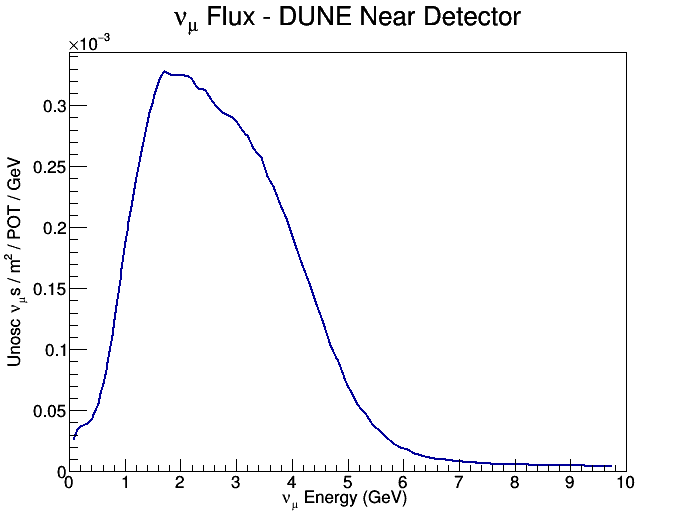
\includegraphics[width=\linewidth]{Dune_Flux/numu_ND_flux.png}
\endminipage
\minipage{.5\textwidth}
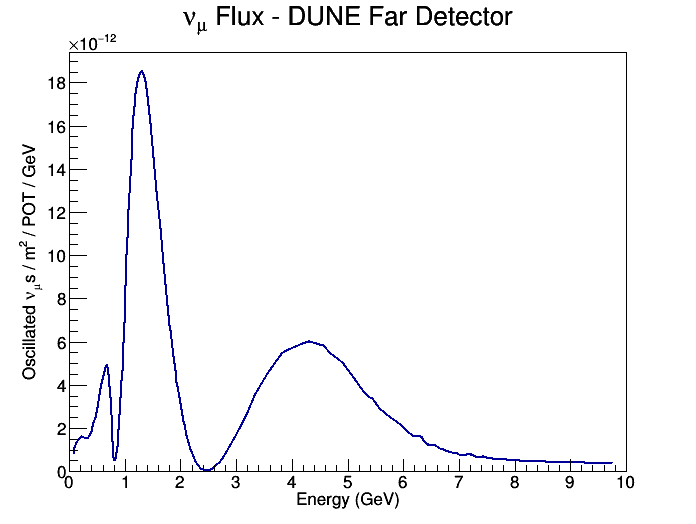
\includegraphics[width=\linewidth]{Dune_Flux/numu_FD_flux.png}
\endminipage
\caption{$\nu_\mu$ flux at DUNE ND (Left) and FD (Right)}
\label{fig:dune_flux}
\end{figure}

\begin{table}
\centering
 \begin{tabular}{| l  c  c |} 
 \hline 
 Parameter & Central Value & Relative Uncertainty\\ [0.5ex] 
 \hline
 $\theta_{12}$ & 0.5843 & 2.3\% \\ 
% \hline
 $\theta_{23}$ (NH) & 0.738 & 5.9\% \\
% \hline
 $\theta_{23}$ (IH) & 0.864 & 4.9\% \\
%  \hline
 $\theta_{13}$ & 0.148 & 2.5\% \\ 
% \hline
 $\Delta m^2_{21}$ & $7.5\times10^{-5} \textrm{eV}^2$ & 2.4\% \\
%  \hline
 $\Delta m^2_{31}$ (NH) & $2.457\times10^{-3} \textrm{eV}^2$ & 2.0\% \\
% \hline
 $\Delta m^2_{31}$ (IH) & $-2.449\times10^{-3} \textrm{eV}^2$ & 1.9\% \\[1ex]
% \hline
% 4 & 545 & 18744 \\
% \hline
% 5 & 88 & 788 \\ [1ex] 
 \hline
\end{tabular}
\caption{The various Monte Carlo event generators used for this work.}
\label{tab:osc}
\end{table}


\FloatBarrier
	%All studies shown look at the effect of differences between the near and the far detector fluxes. However, we also include the different estimated efficiencies of each of the three near detector configurations.
\subsection{How We Study a Near to Far Extrapolation}
\label{subsec:ntf}
The various studies regarding near to far extrapolations are explored using the following procedure. Ratios of either NEUT or NuWro to GENIE - referred to as 'single ratios' - separately at the ND and FD are taken. NEUT and NuWro are both normalized to GENIE to highlight shape differences rather than overall normalization effects. These offer insight into model variations in and how the dependence of ND configuration couple to these variations.
The effect of a near to far extrapolation is approximated by taking a 'double ratio' between the near and far single ratios. To be explicit, these are defined in Equations ~\ref{eq:single_ratio} and ~\ref{eq:double_ratio}, where 'Other MC' refers to either NEUT or NuWro and 'Near' can be replaced by 'Far' in the single ratio. We note this is a crude approximation to give intuition about the problem for just a single reaction process; a fit to the ND spectrum will have multiple reactions in a given topology which can complicate the determination of physics effects for a single reaction.

\begin{equation}
\label{eq:single_ratio}
\textrm{ND Single Ratio} = \frac{\textrm{(Other MC @ Near Detector)}}{\textrm{(GENIE @ Near Detector)}}
\end{equation}

\begin{equation}
\label{eq:double_ratio}
\textrm{Double Ratio} = \frac{\textrm{(ND Single Ratio)}}{\textrm{(FD Single Ratio)}}
\end{equation}

\subsection{Detector Configurations and Efficiencies}
\label{subsec:eff}
These studies highlight the effect of the different efficiencies of the various detectors. We first consider a 'perfect' ND and FD without any efficiencies applied, and then look what changes as we consider the 3 different configurations of the ND and a simple LAr efficiency in the FD. 

Efficiency information is included with the following procedure. Each particle is randomly accepted or rejected by throwing a random number and checking against the efficiency according to the particle's momentum. No angular efficiencies have yet been taken into account for this work. At time of this writing, only a full description of the FGT efficiency according to NDTF samples is available, but other configurations will be added to subsequent versions of this note. An example of the efficiency for protons in the FGT is given in Figure~\ref{fig:FGT_proton_effs}, FGT efficiencies for other particles are included in Appendix~\ref{}. We also lack knowledge of the efficienes for $\pi^0$ in the FGT, so we accept all of these in this configuration. Because we do not have the efficiences for the LAr and GAr, simple thresholds for protons are applied for the GAr - 100 MeV/c - and LAr ND and FD - 200 MeV/c. We also make no assumptions for the efficiencies of $\mu$, $\pi^{+,-}$, and $\pi^{0}$ in the simple  descriptions, and so all of these types of particles are accepted in the LAr and GAr.

\begin{figure}[h]
\centering
\minipage{.5\textwidth}
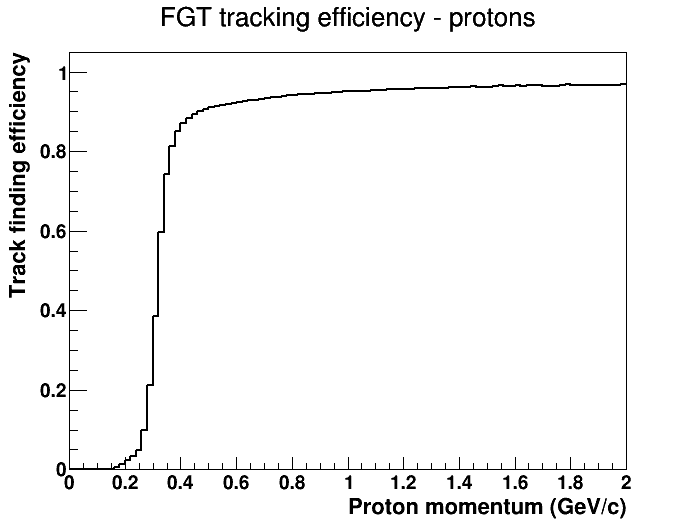
\includegraphics[width=\linewidth]{eff_plots/fgt_trkeff_proton.png}
\endminipage
\minipage{.5\textwidth}
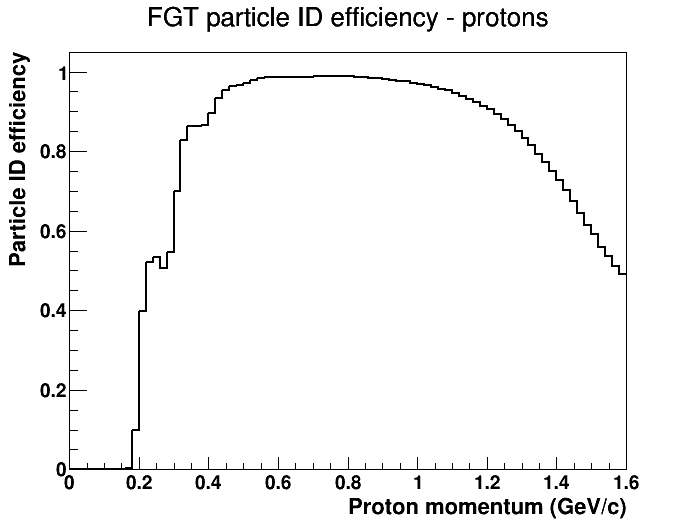
\includegraphics[width=\linewidth]{eff_plots/fgt_pideff_proton.png}
\endminipage
\caption{Left: Tracking efficiency for protons in FGT. Right: PID efficiency for protons in FGT. Total efficiency for a given proton momentum is given by the product of the two efficiencies.}
\label{fig:FGT_proton_effs}
\end{figure}


\section{Parameterization}
%The VALOR group\cite{VALOR} has led multiple T2K oscillation analyses and has contributed to most published T2K oscillation papers(I TOOK THIS ALMOST WORD FOR WORD FROM THE VALOR DOC BUT IDK WHAT TO WRITE FOR IT. IF CITING IT IS NOT GOOD ENOUGH I NEED TO CHANGE THIS). It also has contributed to to optimisation studies for DUNE, this being a source of motivation for this work. 
The VALOR software package has been used on multiple T2K oscillation analyses, and has recently been used to study the DUNE near detector configurations. (((The group uses MC templates to map between reconstructed and true information for various reactions.))) Uncertainties in interaction models are parameterized by model variations as a function of $Q^2$. Currently, $Q^2$ parameterizations are defined for neutrinos and antineutrinos as: 
\begin{itemize}
\item CCQE nm with $Q^2$ bins \{0 - 0.20, 0.20 - 0.55, $>$0.55\} $\textrm{GeV}^2$
\item CCQE nmb with $Q^2$ bins \{0 - 0.20, 0.20 - 0.55, $>$0.55\} $\textrm{GeV}^2$
\item 2p2h nm with 1 $Q^2$ bin 
\item 2p2h nmb with 1 $Q^2$ bin
\end{itemize}

This portion of the work seeks to determine if variations in CCQE and 2p2h models are well represented by these parameterizations in $Q^2$. It also serves to highlight the behavior of the models as they couple to FSI and detector effect as we use a reconstructed $Q^2$ when efficiencies are applied.

\subsection{$Q^2$ Parameterization}
\label{subsec:q2}
%An obvious first step in the investigation of $Q^2$ parameterization sufficiency is to consider the relative change between the models and this change as it is extrapolated between the ND and FD Detector. 
The single and double ratio procedure described in Section~\ref{subsec:ntf} is conducted using events created by all three generators at the ND and FD and distributed according to $Q^2$. This is done separately with and without efficiencies, for both $\nu_{\mu}$ and $\overline{\nu}_{\mu}$, and for true-CCQE and true-2p2h. Applying efficiencies allows us to investigate how the interaction model can couple to detector effects. For distributions without efficiencies, the MC-level $Q^2$ quantity is used, giving us insight into the interaction model uncertainties. However, when including efficiencies, $Q^2$ becomes a reconstructed quantity, as it is calculated from the final state particles that are accepted after efficiencies are applied. This is highlighted in Equations~\ref{eq:Q2} - ~\ref{eq:ereco}. Though we call it 'reconstructed', it is calculated using the true energies and momentums without smearing applied, so it is not truely reconstructed in the usual sense of the word. Using this reconstructed quantity reveals how interaction/FSI variations, and detector effects couple together.

\begin{equation}
\label{eq:Q2}
Q^2 = |q_0^2 - q_3^2|,
\end{equation}
\begin{equation}
\label{eq:q0}
q_0^2 = (E_{reco} - E_{lep})^2,
\end{equation}
\begin{equation}
\label{eq:q3}
q_3^2 = (\vec{P}_{reco} - \vec{P}_{lep})^2
\end{equation}
\begin{equation}
E_{reco} =E_{lep} + \Sigma E_{\pi} + \Sigma (E_{prot} - M_{prot})
\label{eq:ereco}
\end{equation}
Conclusions are drawn from the double ratios according to the following prescription. We look for if the ratio is flat - i.e. if a horizontal line is within the statistical error bars - in a given bin of the parameterization. Flatness in that bin is a crude estimation for model-dependent shape uncertainties canceling out in a near-to-far extrapolation, and shows that a reweighting of that whole bin is sufficient to cover uncertainties. Again, we stress that this is a crude approximation to the near-to-far extrapolation.
 
%, true-2p2h, CC0$\pi^{\pm}$, CC1$\pi^{\pm}$, and CCOther as defined in Section~\ref{subsec:EDiff}

For $\nu_{\mu}$ CCQE events, both NEUT's and NuWro's models differ significantly from GENIE' model in $Q^2$ distributions, as seen in the single ratios in Figure~\ref{fig:Q2_ccqe_no_eff}. Despite this, the double ratios for both NEUT and NuWro to GENIE remain relatively flat and close to 1, with small amounts of variation in the higher $Q^2$ region.

For double ratios with FGT efficiencies applied to the ND and simple LAr efficiencies applied to the FD, shape variations are greater above ~1.25 $\textrm{GeV}^2$ as seen in Figure~\ref{fig:Q2_ccqe_FGT_eff}. This suggests an additional bin in the region .55 to 1.25 $\textrm{GeV}^2$ should be included. These studies will be expanded in the future to increase statistics and determine the origin of the variation in this region, one possible source being the rejection of low-momentum muons after we apply efficiencies.

\begin{figure}[h]
\minipage{.32\textwidth}
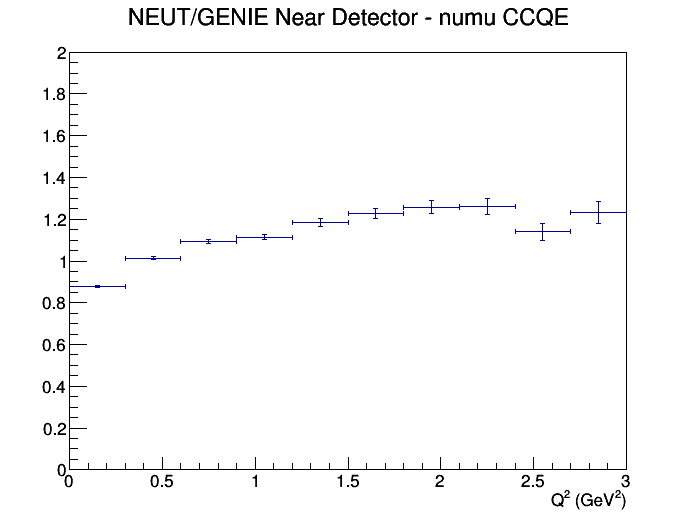
\includegraphics[width=\linewidth]{Q2/nominal/ratios/CCQE_NEUT_GENIE_numu_near_Q2.png}
\endminipage
\minipage{.32\textwidth}
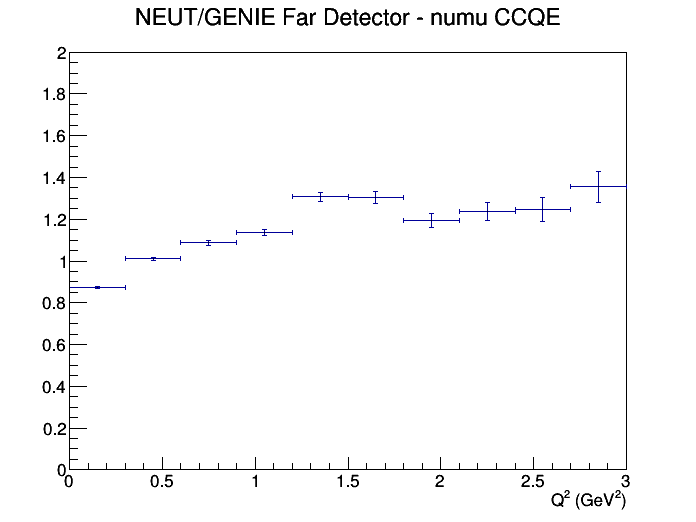
\includegraphics[width=\linewidth]{Q2/nominal/ratios/CCQE_NEUT_GENIE_numu_far_Q2.png}
\endminipage
\minipage{.32\textwidth}
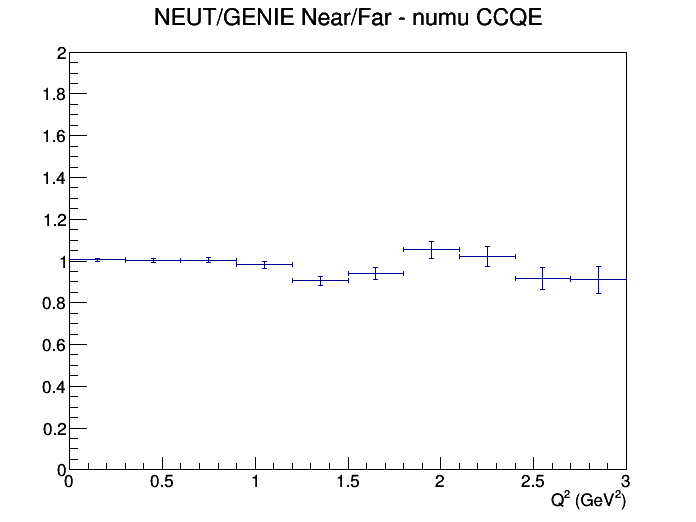
\includegraphics[width=\linewidth]{Q2/nominal/ratios/CCQE_NEUT_GENIE_numu_NF_Q2.png}
\endminipage
\newline
\minipage{.32\textwidth}
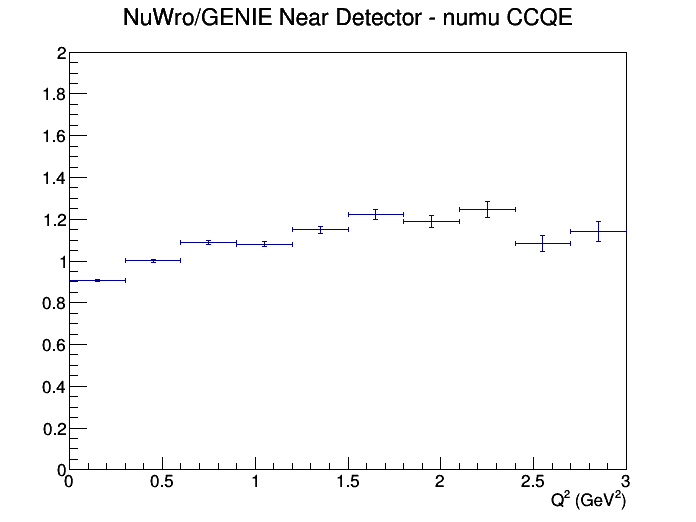
\includegraphics[width=\linewidth]{Q2/nominal/ratios/CCQE_NuWro_GENIE_numu_near_Q2.png}
\endminipage
\minipage{.32\textwidth}
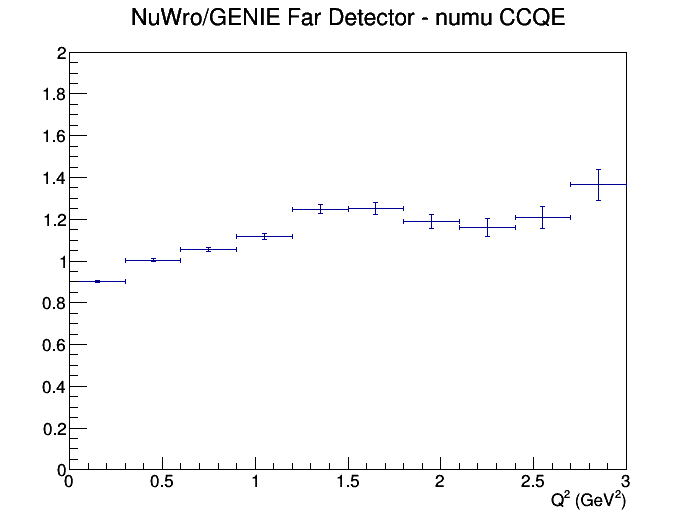
\includegraphics[width=\linewidth]{Q2/nominal/ratios/CCQE_NuWro_GENIE_numu_far_Q2.png}
\endminipage
\minipage{.32\textwidth}
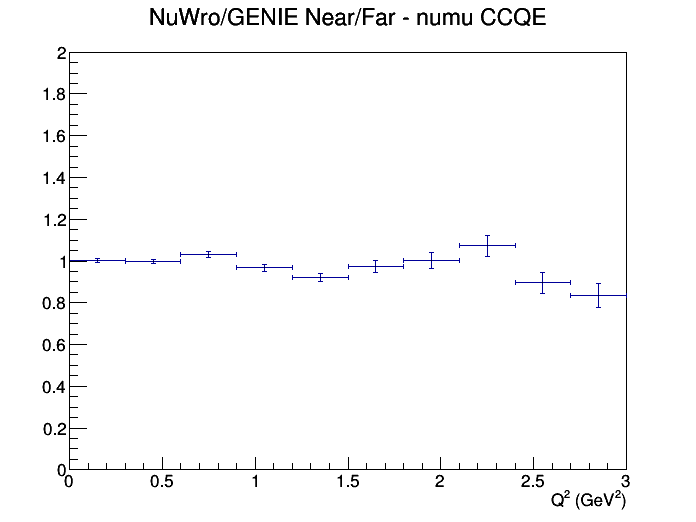
\includegraphics[width=\linewidth]{Q2/nominal/ratios/CCQE_NuWro_GENIE_numu_NF_Q2.png}
\endminipage
\caption{MC-level $Q^2$ distributed $\nu_{\mu}$ events using DUNE flux, no efficiencies applied to ND or FD. Top: Ratios of NEUT to GENIE. Bottom: Ratios of NuWro to GENIE. Left to Right: Single ratio at ND, single ratio at FD, double ratio Near/Far. Of note is the relative flatness throughout the double ratio compared to the single ratio at the ND. Note that the VALOR binning is separated by lower bin edges of (0, 0.20, and 0.55) $\textrm{GeV}^2$}
\label{fig:Q2_ccqe_no_eff}
\end{figure}
\begin{figure}[h]
\minipage{.32\textwidth}
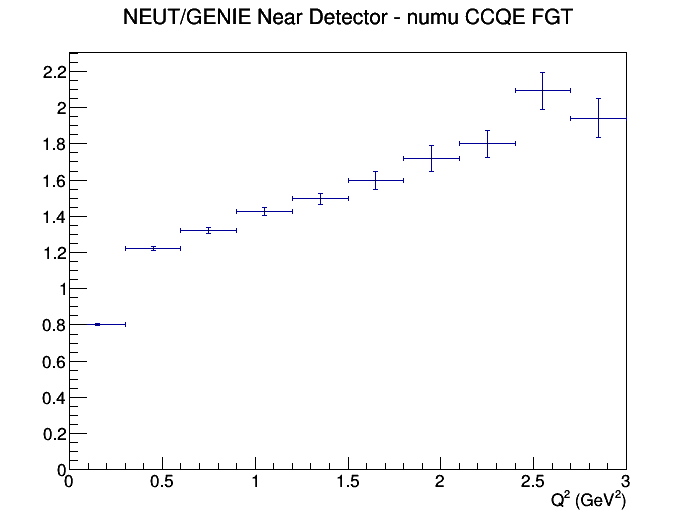
\includegraphics[width=\linewidth]{eff_Q2/FGT/ratios/CCQE_NEUT_GENIE_numu_near_Q2.png}
\endminipage
\minipage{.32\textwidth}
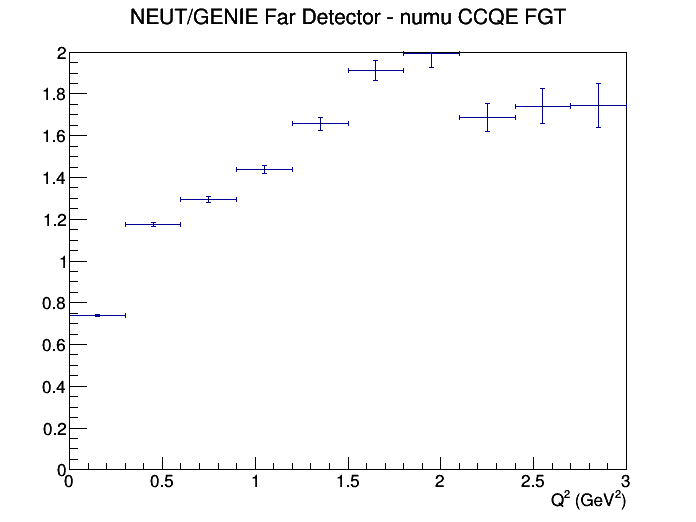
\includegraphics[width=\linewidth]{eff_Q2/FGT/ratios/CCQE_NEUT_GENIE_numu_far_Q2.png}
\endminipage
\minipage{.32\textwidth}
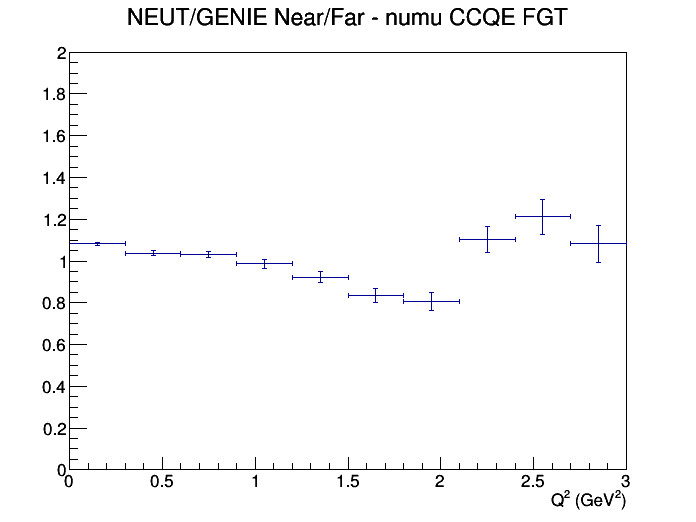
\includegraphics[width=\linewidth]{eff_Q2/FGT/ratios/CCQE_NEUT_GENIE_numu_NF_Q2.png}
\endminipage
\newline
\minipage{.32\textwidth}
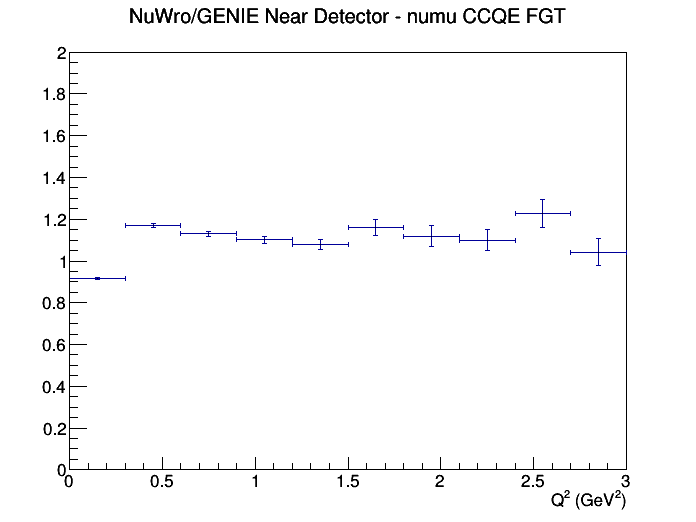
\includegraphics[width=\linewidth]{eff_Q2/FGT/ratios/CCQE_NuWro_GENIE_numu_near_Q2.png}
\endminipage
\minipage{.32\textwidth}
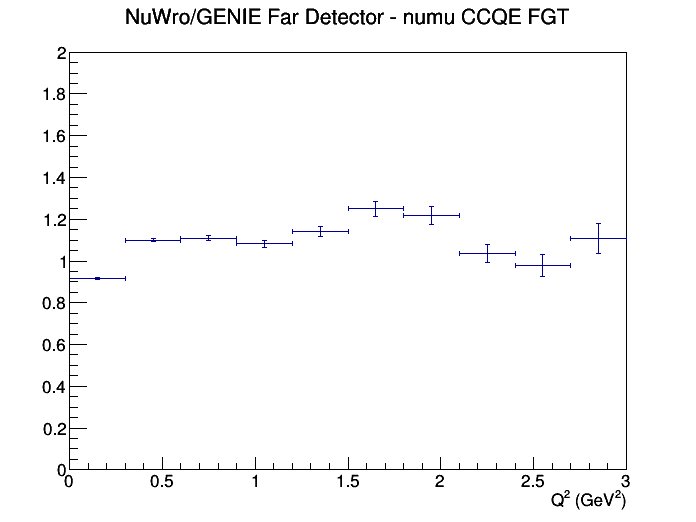
\includegraphics[width=\linewidth]{eff_Q2/FGT/ratios/CCQE_NuWro_GENIE_numu_far_Q2.png}
\endminipage
\minipage{.32\textwidth}
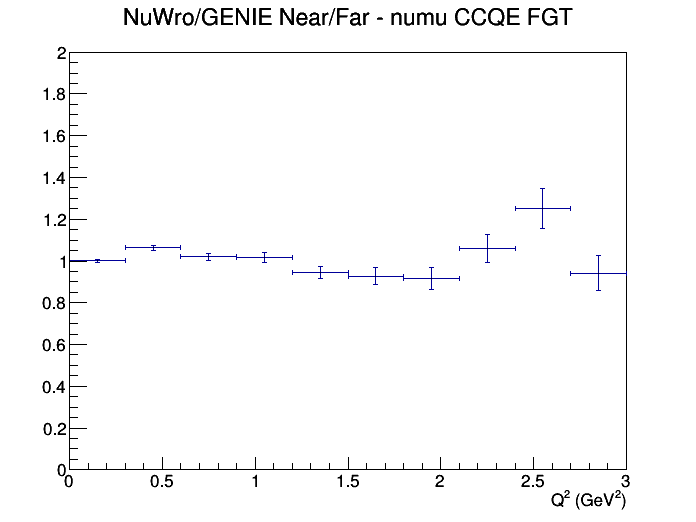
\includegraphics[width=\linewidth]{eff_Q2/FGT/ratios/CCQE_NuWro_GENIE_numu_NF_Q2.png}
\endminipage
\caption{Reconstructed $Q^2$ distributed $\nu_{\mu}$ events using DUNE flux, FGT efficiencies applied to ND and simple LAr effiencies applied to FD. Top: Ratios of NEUT to GENIE. Bottom: Ratios of NuWro to GENIE. Left to Right: Single ratio at ND, single ratio at FD, double ratio Near/Far. More shape variations do arise above around 1.25 $\textrm{GeV}^2$ in the double ratios. This suggests another bin should encompass the region between .55 and 1.25 $\textrm{GeV}^2$. Note that the current VALOR binning is separated by lower bin edges of (0, 0.20, and 0.55) $\textrm{GeV}^2$}
\label{fig:Q2_ccqe_FGT_eff}
\end{figure}
\FloatBarrier


However, for $\overline{\nu}_{\mu}$ CCQE events, we observe distortions in the $Q^2$ distribution even in the double ratios. This is true without efficiencies for both NEUT to GENIE and NuWro to GENIE ratios. This is displayed in Figure~\ref{fig:Q2_ccqe_bar}. The variations again arise above 1.5 $\textrm{GeV}^2$ for the double ratios, supporting the addition of a bin between .55 and 1.25 $\textrm{GeV}^2$. This appears without efficiencies, and points to variations in the CCQE interaction model being responsible for this effect rather than FSI variations or detector effects.

We run into trouble extending the $\overline{\nu}_{\mu}$ CCQE study with efficiencies applied, as this leaves the high $Q^2$ region with very low statistics, preventing us from drawing any meaningful conclusions. These plots are included in Appendix~\ref{app:Q2_app} for completeness. The studies will be continued once we have higher statistics, and with more complete descriptions of the LAr and GAr as this information becomes available.

\begin{figure}[h]
\minipage{.32\textwidth}
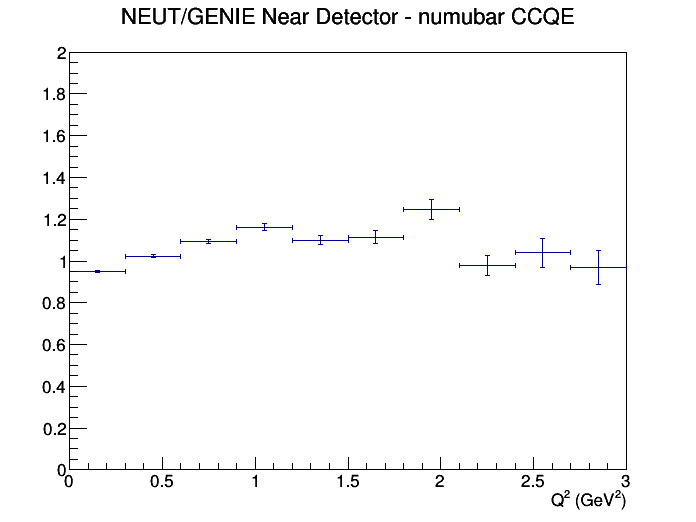
\includegraphics[width=\linewidth]{Q2/nominal/ratios/CCQE_NEUT_GENIE_numubar_near_Q2.png}
\endminipage
\minipage{.32\textwidth}
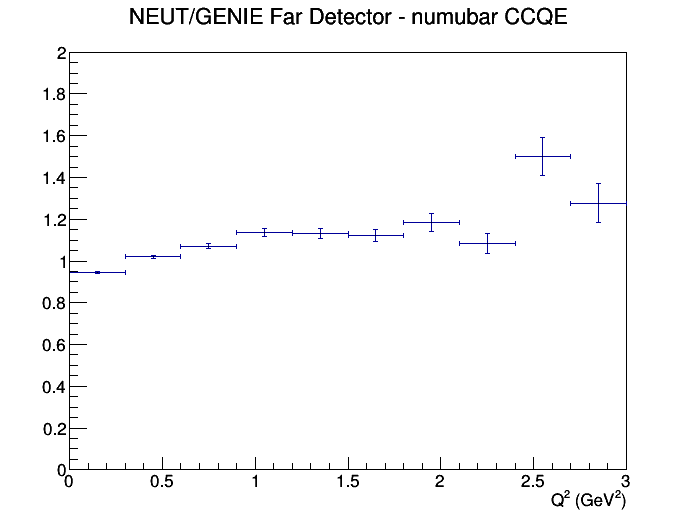
\includegraphics[width=\linewidth]{Q2/nominal/ratios/CCQE_NEUT_GENIE_numubar_far_Q2.png}
\endminipage
\minipage{.32\textwidth}
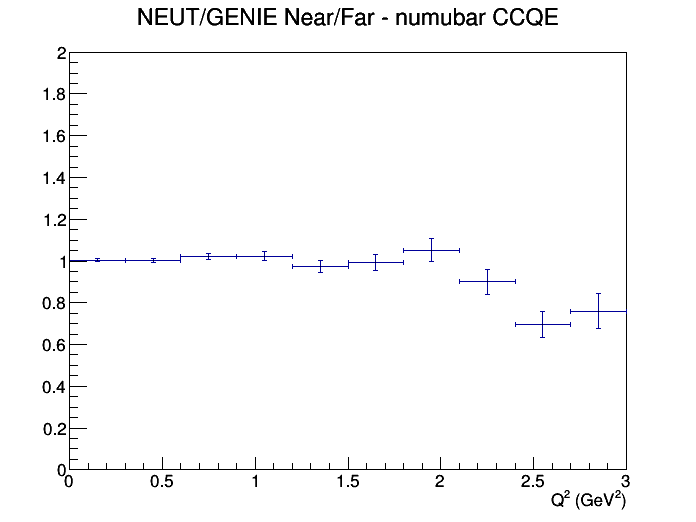
\includegraphics[width=\linewidth]{Q2/nominal/ratios/CCQE_NEUT_GENIE_numubar_NF_Q2.png}
\endminipage
\newline
\minipage{.32\textwidth}
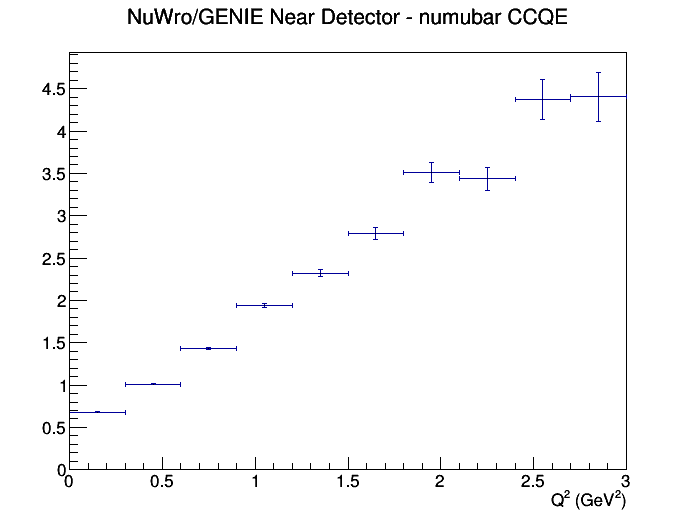
\includegraphics[width=\linewidth]{Q2/nominal/ratios/CCQE_NuWro_GENIE_numubar_near_Q2.png}
\endminipage
\minipage{.32\textwidth}
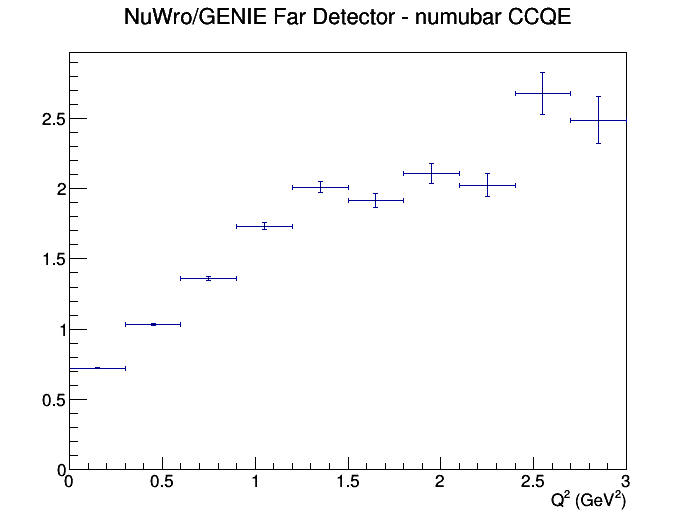
\includegraphics[width=\linewidth]{Q2/nominal/ratios/CCQE_NuWro_GENIE_numubar_far_Q2.png}
\endminipage
\minipage{.32\textwidth}
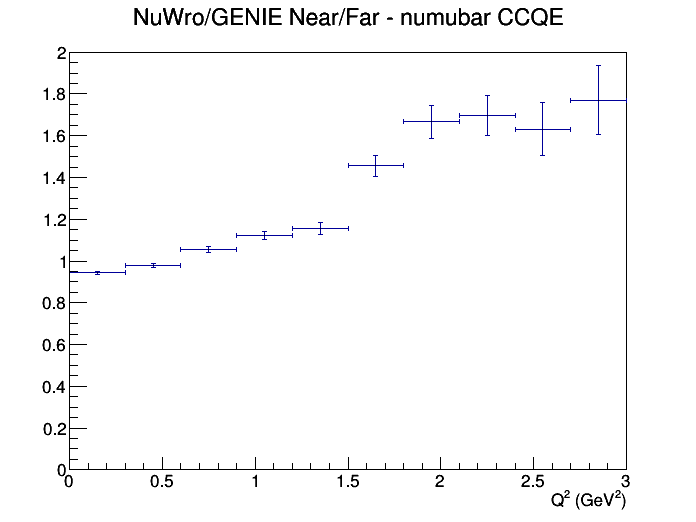
\includegraphics[width=\linewidth]{Q2/nominal/ratios/CCQE_NuWro_GENIE_numubar_NF_Q2.png}
\endminipage
\caption{MC-level $Q^2$ distributed $\overline{\nu}_{\mu}$ CCQE events using DUNE flux. Top: Ratios of NEUT to GENIE. Bottom: Ratios of NuWro to GENIE. Left to Right: Single ratio at ND, single ratio at FD, double ratio Near/Far. Large amounts of variations in the region above 1.5 $\textrm{GeV}^2$ in both double ratios. This differs from $\nu_{\mu}$ CCQE, where this arose in the ratios after efficiencies are added. Here, it exists without any efficiencies, pointing to variations in the CCQE model, rather than FSI or detector effects, not being covered by the parameterization. An additional bin between .55 and 1.25 $\textrm{GeV}^2$ is suggested. Note that the VALOR binning is separated by lower bin edges of (0, 0.20, and 0.55) $\textrm{GeV}^2$.}
\label{fig:Q2_ccqe_bar}
\end{figure}
\FloatBarrier

For 2p2h $\nu_{\mu}$ and $\overline{\nu}_{\mu}$ events, the double ratios from both NEUT and NuWro remain centered close to or around 1 below about 1 $\textrm{GeV}^2$ without efficiencies applied, as seen in Figure~\ref{fig:Q2_2p2h_numu_no_eff} and ~\ref{fig:Q2_2p2h_numubar_no_eff}. Above 1 $\textrm{GeV}^2$, the statistics are again low. At this moment, the currently-proposed 1-bin normalization appears sufficient in the region below 1 $\textrm{GeV}^2$. The low statistics prevent us from making conclusions in the high $Q^2$ region as well as drawing conclusions from applying efficiencies. These will be revisted in later iterations of this work.
\begin{figure}[h]
\minipage{.32\textwidth}
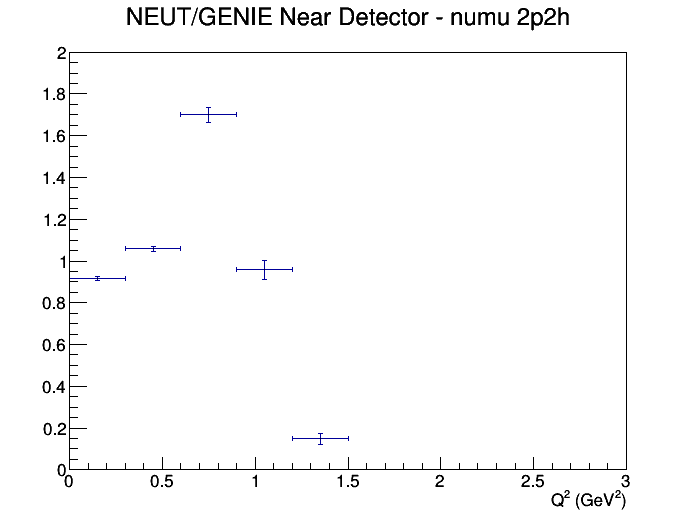
\includegraphics[width=\linewidth]{Q2/nominal/ratios/2p2h_NEUT_GENIE_numu_near_Q2.png}
\endminipage
\minipage{.32\textwidth}
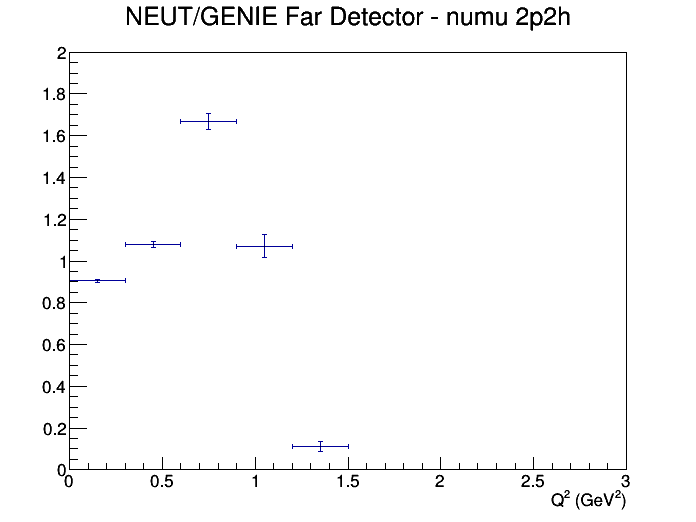
\includegraphics[width=\linewidth]{Q2/nominal/ratios/2p2h_NEUT_GENIE_numu_far_Q2.png}
\endminipage
\minipage{.32\textwidth}
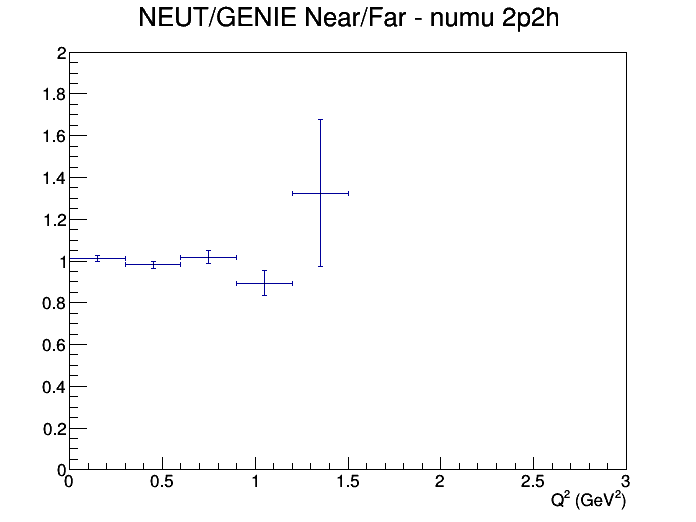
\includegraphics[width=\linewidth]{Q2/nominal/ratios/2p2h_NEUT_GENIE_numu_NF_Q2.png}
\endminipage
\newline
\minipage{.32\textwidth}
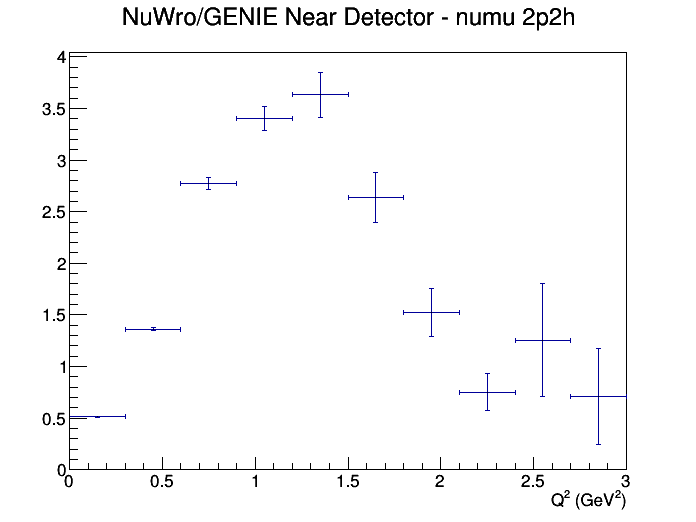
\includegraphics[width=\linewidth]{Q2/nominal/ratios/2p2h_NuWro_GENIE_numu_near_Q2.png}
\endminipage
\minipage{.32\textwidth}
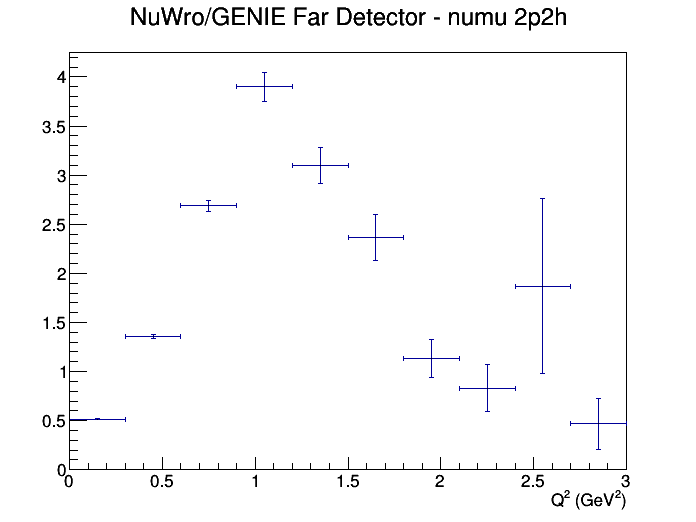
\includegraphics[width=\linewidth]{Q2/nominal/ratios/2p2h_NuWro_GENIE_numu_far_Q2.png}
\endminipage
\minipage{.32\textwidth}
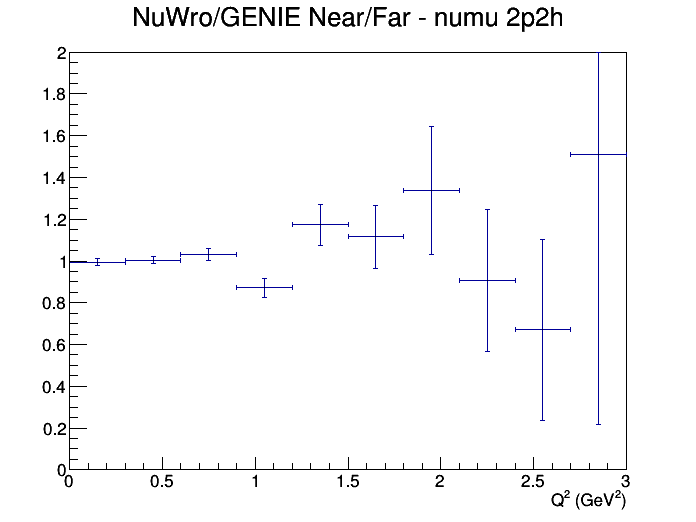
\includegraphics[width=\linewidth]{Q2/nominal/ratios/2p2h_NuWro_GENIE_numu_NF_Q2.png}
\endminipage
\caption{$Q^2$ distributed $\overline{\nu}_{\mu}$ 2p2h events using DUNE flux. Top: Ratios of NEUT to GENIE. Bottom: Ratios of NuWro to GENIE. Left to Right: Single ratio at ND, single ratio at FD, double ratio Near/Far. Large amounts of variations are present resulting from low statistics in the higher end of all distributions, but the lower end holds close to 1. Note that the VALOR binning is separated by lower bin edges of (0, 0.20, and 0.55) $\textrm{GeV}^2$.}
\label{fig:Q2_2p2h_numu_no_eff}
\end{figure}

\begin{figure}[h]
\minipage{.32\textwidth}
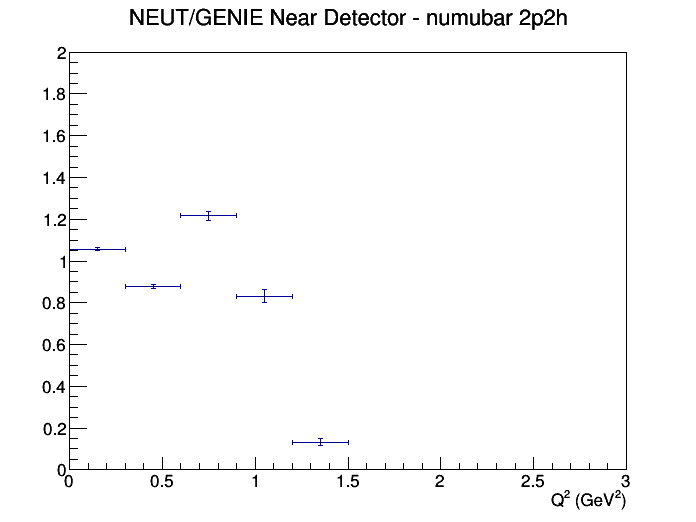
\includegraphics[width=\linewidth]{Q2/nominal/ratios/2p2h_NEUT_GENIE_numubar_near_Q2.png}
\endminipage
\minipage{.32\textwidth}
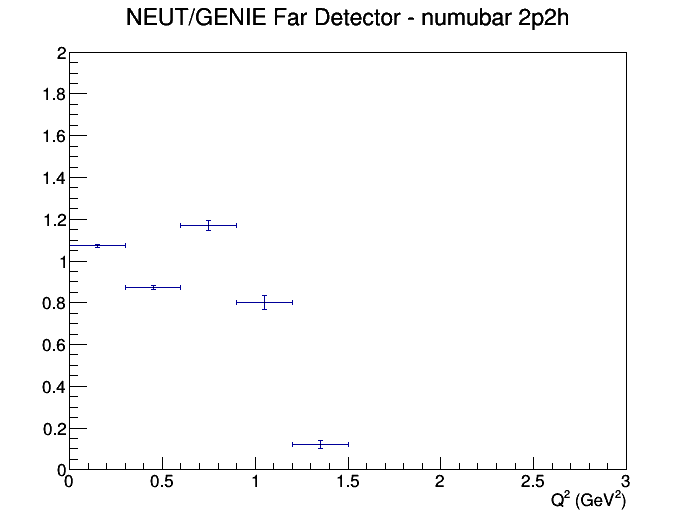
\includegraphics[width=\linewidth]{Q2/nominal/ratios/2p2h_NEUT_GENIE_numubar_far_Q2.png}
\endminipage
\minipage{.32\textwidth}
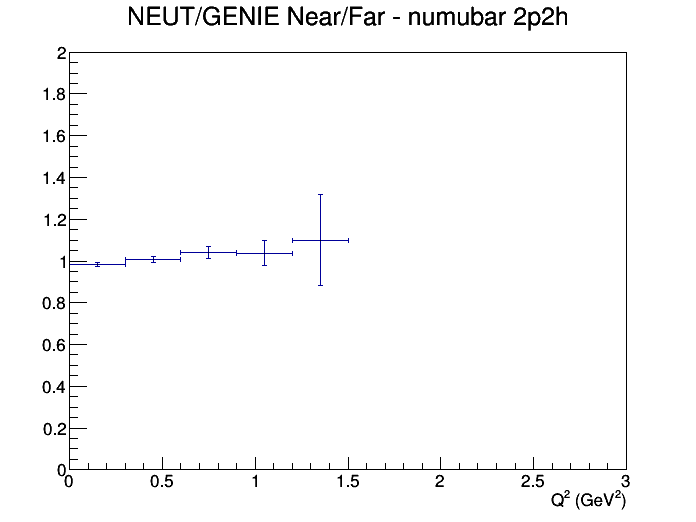
\includegraphics[width=\linewidth]{Q2/nominal/ratios/2p2h_NEUT_GENIE_numubar_NF_Q2.png}
\endminipage
\newline
\minipage{.32\textwidth}
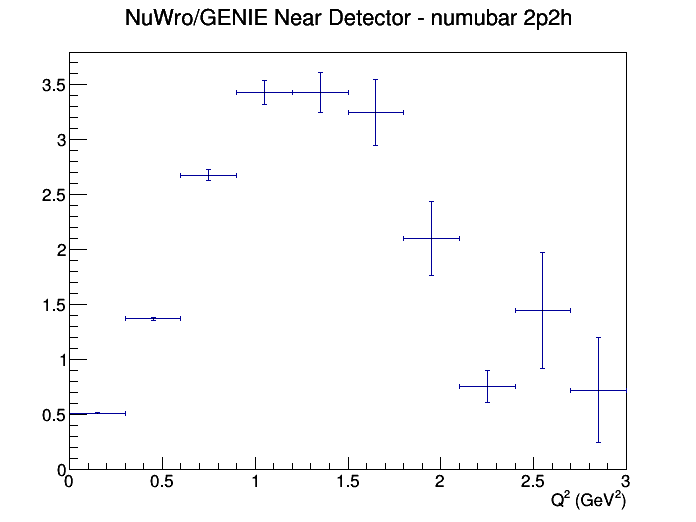
\includegraphics[width=\linewidth]{Q2/nominal/ratios/2p2h_NuWro_GENIE_numubar_near_Q2.png}
\endminipage
\minipage{.32\textwidth}
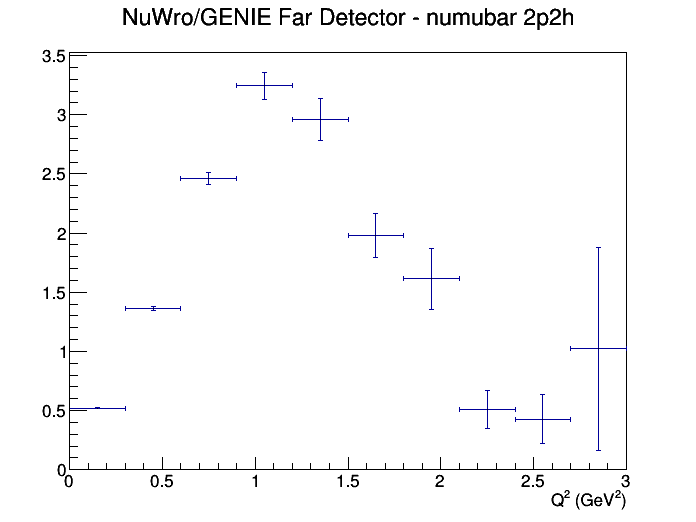
\includegraphics[width=\linewidth]{Q2/nominal/ratios/2p2h_NuWro_GENIE_numubar_far_Q2.png}
\endminipage
\minipage{.32\textwidth}
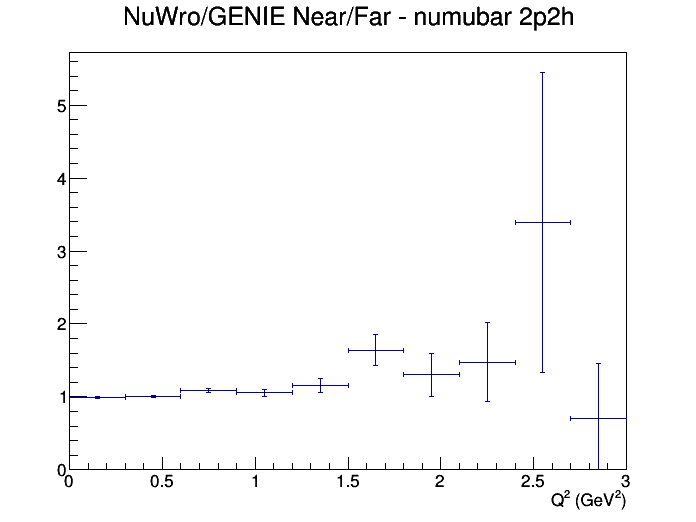
\includegraphics[width=\linewidth]{Q2/nominal/ratios/2p2h_NuWro_GENIE_numubar_NF_Q2.png}
\endminipage
\caption{$Q^2$ distributed $\overline{\nu}_{\mu}$ 2p2h events using DUNE flux. Top: No efficiences, Bottom: FGT efficiencies applied to ND, LAr efficiencies applied to FD. Left to right: NEUT to GENIE double ratio, NuWro to GENIE double ratio. Large amounts of deviations from 1 throughout distributions with efficiencies applied. Note that the VALOR binning is separated by lower bin edges of (0, 0.20, and 0.55) $\textrm{GeV}^2$.}
\label{fig:Q2_2p2h_numubar_no_eff}
\end{figure}
\FloatBarrier

We currently find an additional bin in the region (.55, ~1.25) will account for uncertainties in both $\nu_{\mu}$ and $\overline{\nu}_{\mu}$ CCQE. For $\nu_{\mu}$ and $\overline{\nu}_{\mu}$ 2p2h, the overall normalization currently appears sufficient from these studies. Investigations into the origin of the variation in the high $Q^2$ region of CCQE will be conducted as this work is furthered. Additional statistics and more complete effiency descriptions for the LAr and GAr are required, and will be conducted at a later date.

\subsection{$q_0 \textrm{ vs. } q_3$ Variations}
\label{subsec:q0q3}
In addition to studying the $Q^2$ ratios, the ratios in $q_0 \textrm{ - } q_3$ were also investigated to explore the possibility that variations arrise when changing the parameterization from $Q^2$ to $q_0 \textrm{ - } q_3$. The $Q^2$ parameterization assumes the variations are purely functions of $Q^2$. Under this assumption, the double ratios should be flat in $q_0 \textrm{ - } q_3$ regions corresponding to the $Q^2$-binned parameterization. If this is not the case, a pure-$Q^2$ parameterization cannot sufficiently account for CCQE and 2p2h variations. 

These studies were done in the exact same way as those in the previous section, only with the events and ratios distributed in $q_0 \textrm{ - } q_3$ bins. Note: to be symmetric arround 1, the scale extends from 0 to 2, but the variations in those bins can actually be greater than 2. Again, the quantities are MC-level truth information in the distributions without efficiencies, but are reconstructed in those with effiencies applied, as described in Equations~\ref{eq:Q2} - ~\ref{eq:ereco}.

For $\nu_{\mu}$ CCQE, the double ratios without efficiencies appear flat for both NEUT to GENIE and NuWro to GENIE double ratios, as seen in Figure~\ref{fig:q0q3_numu_CCQE_no_eff}. There is distortion in the upper right region, consistent with the high $Q^2$ regions in Figure~\ref{fig:Q2_ccqe_no_eff}.  This binning proves to be a problem for creating reliable conclusions once efficiencies are applied, as statistics for each individual bin become quite low. These are included in Appendix~\ref{q0q3_app}. Higher statistics will be achieved for future work.
%\newline
\begin{figure}[h]
\centering
\minipage{.5\textwidth}
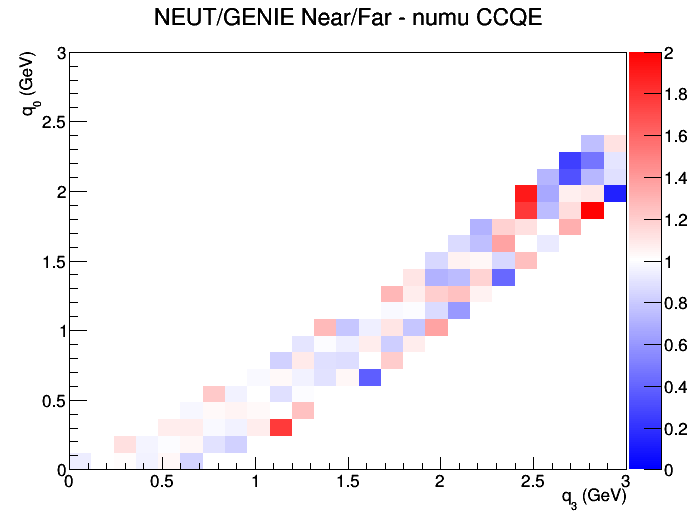
\includegraphics[width=\linewidth]{q0_q3/nominal/ratios/CCQE_NEUT_GENIE_numu_NF_q3_q0.png}
\endminipage
\minipage{.5\textwidth}
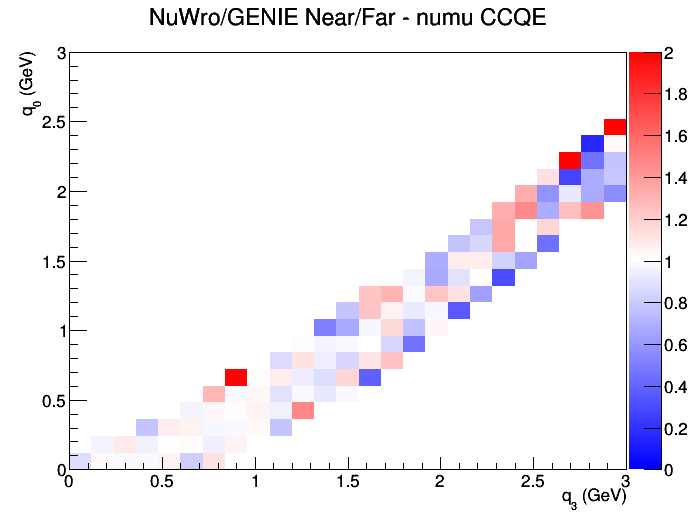
\includegraphics[width=\linewidth]{q0_q3/nominal/ratios/CCQE_NuWro_GENIE_numu_NF_q3_q0.png}
\endminipage
\caption{MC-level $q_0 \textrm{ - } q_3$ distributed $\nu_{\mu}$ CCQE events using DUNE flux without efficiencies applied. Left: Double ratio of NEUT to GENIE, Right: Double ratio of NuWro to GENIE. Relatively flat distributions, but with bin-to-bin variations arising from low statistics. Consistent with corresponding $Q^2$ ratios} 
\label{fig:q0q3_numu_CCQE_no_eff}
\end{figure}
\FloatBarrier

For $\overline{\nu}_{\mu}$ CCQE, the large variations in the high $Q^2$ region are present in the corresponding $q_0 \textrm{ - } q_3$region. As shown in Figure~\ref{fig:q0q3_numubar_CCQE_no_eff}, the upper right region of both double ratios are consistent with the corresponding double ratios in Figure~\ref{fig:Q2_ccqe_bar}. Here again, the NuWro to GENIE double ratio is consistently higher in this region, while the NEUT to GENIE double ratio is slightly lower.

\begin{figure}[h]
\centering
\minipage{.5\textwidth}
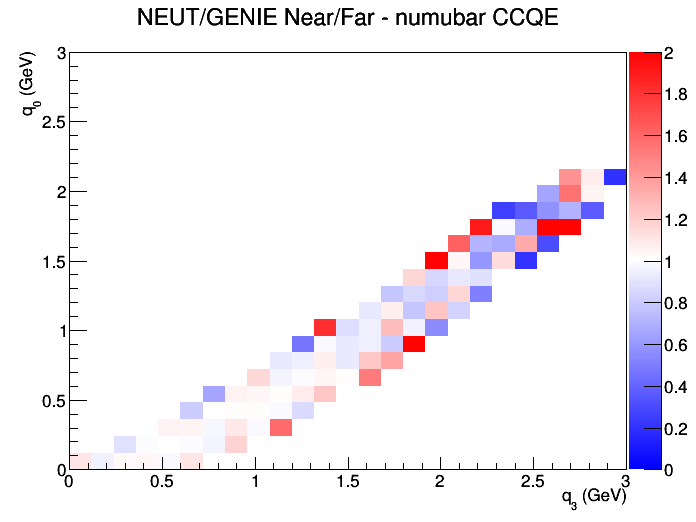
\includegraphics[width=\linewidth]{q0_q3/nominal/ratios/CCQE_NEUT_GENIE_numubar_NF_q3_q0.png}
\endminipage
\minipage{.5\textwidth}
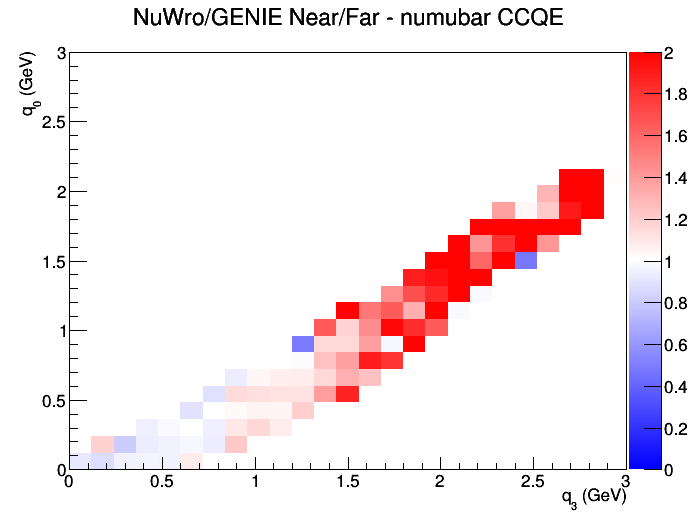
\includegraphics[width=\linewidth]{q0_q3/nominal/ratios/CCQE_NuWro_GENIE_numubar_NF_q3_q0.png}
\endminipage
\caption{$q_0 \textrm{ - } q_3$ distributed $\overline{\nu}_{\mu}$ CCQE events using DUNE flux without efficiencies applied. Left: Double ratio of NEUT to GENIE, Right: Double ratio of NuWro to GENIE. Variations in upper right region. Consistent with corresponding $Q^2$ ratios.}
\label{fig:q0q3_numubar_CCQE_no_eff}
\end{figure}
\FloatBarrier

Each of the three generators have very different behavior for 2p2h $\nu_\mu$ and $\overline{\nu}_{\mu}$ events with no efficiencies applied, as can be seen in Figure~\ref{fig:q0q3_2p2h_events}. This contains the raw event rate for 2p2h, and is shown to highlight the drastic shape difference. This causes very restriced phase space in the double ratios in $q_0 \textrm{ - } q_3$, and so double ratios are not shown here - however they are included in ~\ref{app:q0q3_app}. The shape differences suggest that an overall binning in $Q^2$ cannot cover uncertainties, and reweighting events according to $q_0 \textrm{ - } q_3$ shape should be used instead.
\begin{figure}[h]
\centering
\minipage{.32\textwidth}
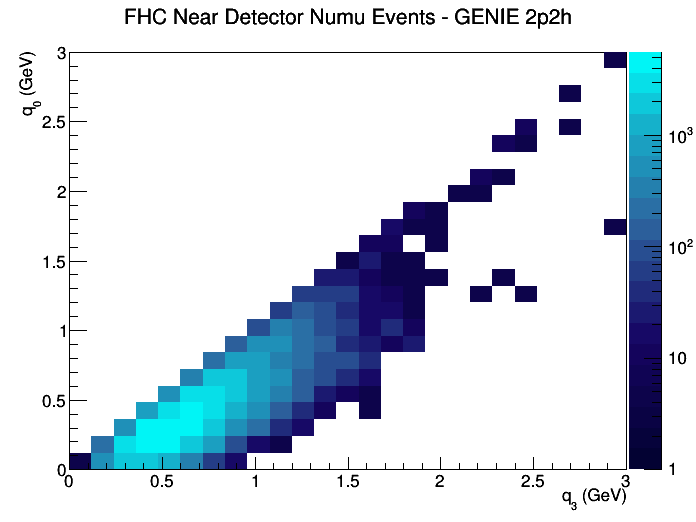
\includegraphics[width=\linewidth]{q0_q3/nominal/2p2h_FHC_ND_numu_q3_q0_GENIE.png}
\endminipage
\minipage{.32\textwidth}
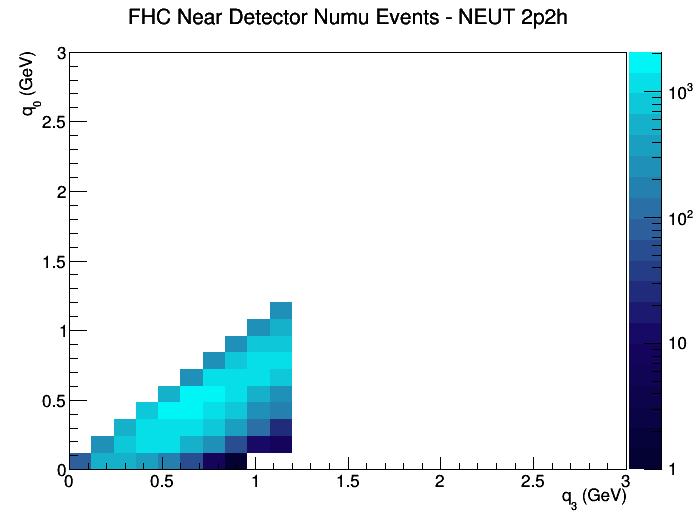
\includegraphics[width=\linewidth]{q0_q3/nominal/2p2h_FHC_ND_numu_q3_q0_NEUT.png}
\endminipage
\minipage{.32\textwidth}
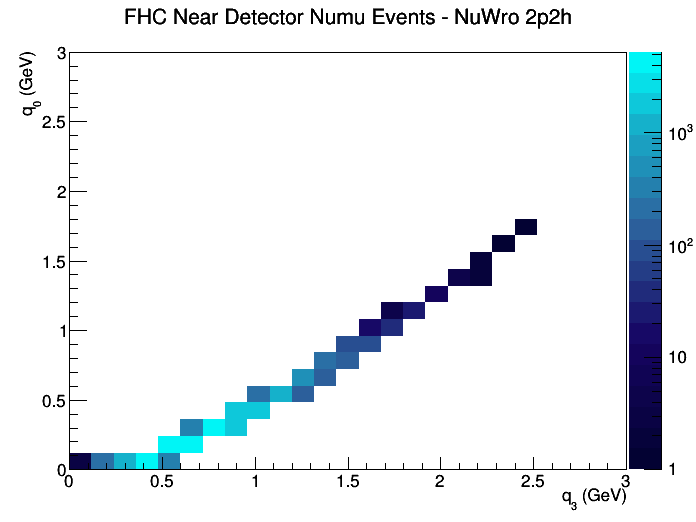
\includegraphics[width=\linewidth]{q0_q3/nominal/2p2h_FHC_ND_numu_q3_q0_NuWro.png}
\endminipage
\newline
\minipage{.32\textwidth}
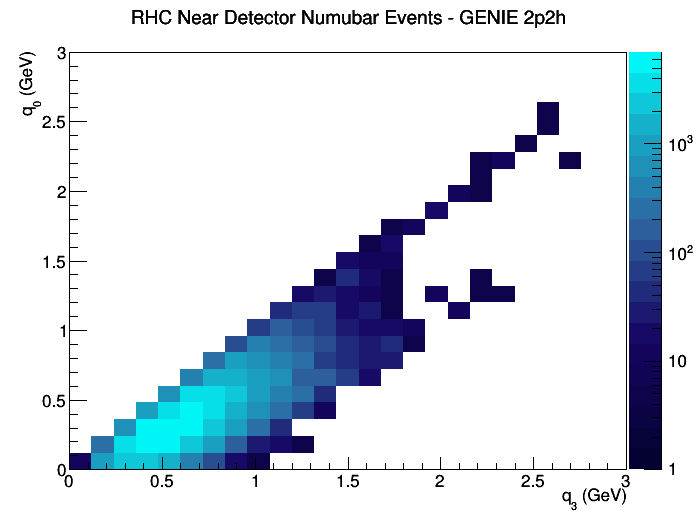
\includegraphics[width=\linewidth]{q0_q3/nominal/2p2h_RHC_ND_numubar_q3_q0_GENIE.png}
\endminipage
\minipage{.32\textwidth}
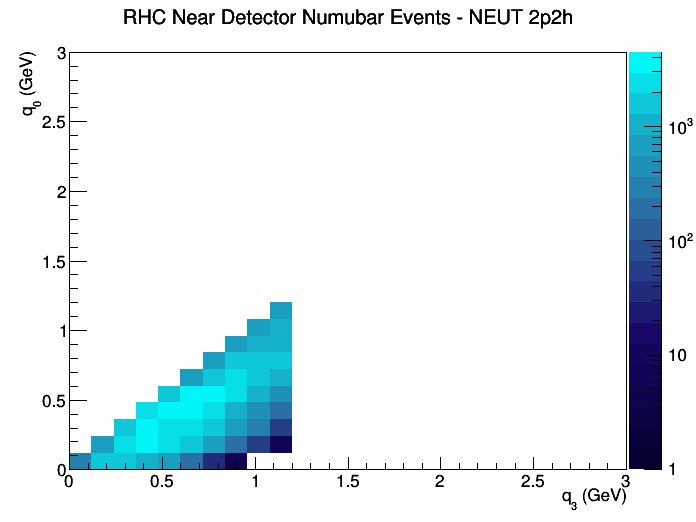
\includegraphics[width=\linewidth]{q0_q3/nominal/2p2h_RHC_ND_numubar_q3_q0_NEUT.png}
\endminipage
\minipage{.32\textwidth}
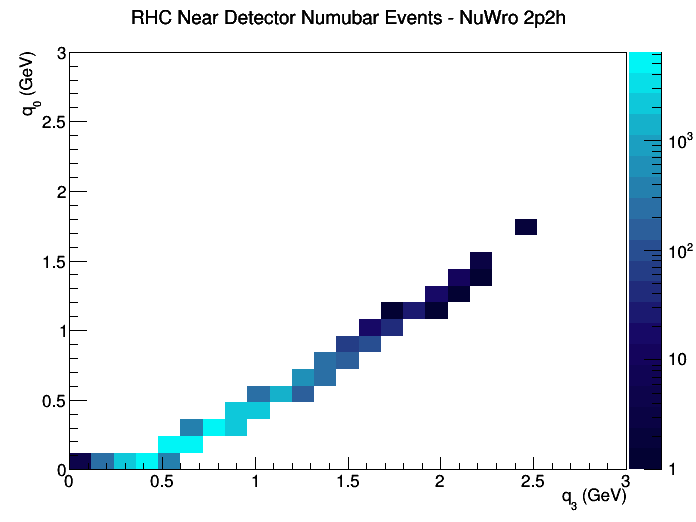
\includegraphics[width=\linewidth]{q0_q3/nominal/2p2h_RHC_ND_numubar_q3_q0_NuWro.png}
\endminipage
\caption{MC-level $q_0 \textrm{ - } q_3$ distributed 2p2h events using DUNE flux with no efficiencies applied. Top: $\nu_{\mu}$ events, Bottom: $\overline{\nu}_{\mu}$ events. Right to Left: GENIE events distribution, NEUT events distribution, NuWro events distribution. The phase spaces are very different without efficiencies, and restrict the coverage of the double ratios in $q_0 \textrm{ - } q_3$. Suggest use of 1 $Q^2$ bin to cover uncertainties.}
\label{fig:q0q3_2p2h_events}
\end{figure}
\FloatBarrier

\subsection{Parameterization - Conclusions}
It appears as though the pure-$Q^2$ paramterization and the binning developed by VALOR would cover model variations for $\nu_{\mu}$ and $\overline{\nu}_{\mu}$ CCQE events, but slight modifications are suggested. The near-to-far extrapolation plots - the double ratios - appear relatively flat in the regions of the individual bins in the low $Q^2$ region. This changes above ~1.25 $\textrm{GeV}^2$, so placing another bin between 0.55 and ~1.25 $\textrm{GeV}^2$ should suffice. The $q_0 \textrm{ - } q_3$ double ratios are consistent with this conclusion. Future work will be focused on improving statistics and implementing full LAr and GAr efficiencies as that information becomes available, as well as investigating the origin of the high-$Q^2$ variations which possibly arise from proton or - more-likely - muon acceptance effects. 

The low-$Q^2$ $\nu_{\mu}$ and $\overline{\nu}_{\mu}$ 2p2h events appear to be covered by the current 1-bin parameterization when only looking at the $Q^2$ distribution. However, the shape differences in $q_0 \textrm{ - } q_3$ show that a pure-$Q^2$ parameterization should not be used. Future work will continue with improving statistics, as well as implementing all efficiencies.

%There is a degree of statistical limitation of the studies at this point, evident in the presence of bin-to-bin variations. To explore this point further, these studies can quickly and easily be extended to larger data sets to deal with statistics limitations. Additionally, the statistical uncertainties in the single and double ratios will also be investigated. With these, we can move on to quantify the degree to which the near-to-far extrapolation covers variations in the $\nu_{\mu}$ case - or does not cover variations in the $\overline{\nu}_{\mu}$ case. 

%For the rest of the reaction modes, the trend - that $\nu_{\mu}$ ratios appear to be relatively flat for both NEUT and NuWro, while $\overline{\nu}_{\mu}$ NuWro to GENIE double ratio is noticeably greater than 1 - continues. This can be seen in Appendix~\ref{app:q0q3_app}. Of note, however, is the shape of $\nu_\mu$ and $\overline{\nu}_{\mu}$ CCOther events before and after efficiencies are applied in each generator. As shown in Figure~\ref{fig:q0q3_numu_CCOther_events}, the left region of $q_0 \textrm{ - } q_3$ space is empty before efficiencies, but is filled in after efficiencies are applied. This corresponds to a low $Q^2$ region, which is shown to be filled in after efficiencies in the $Q^2$ distribution in Figure~\ref{fig:Q2_numu_CCOther_events}.
%\begin{figure}[h]
%\centering
%\minipage{.3\textwidth}
%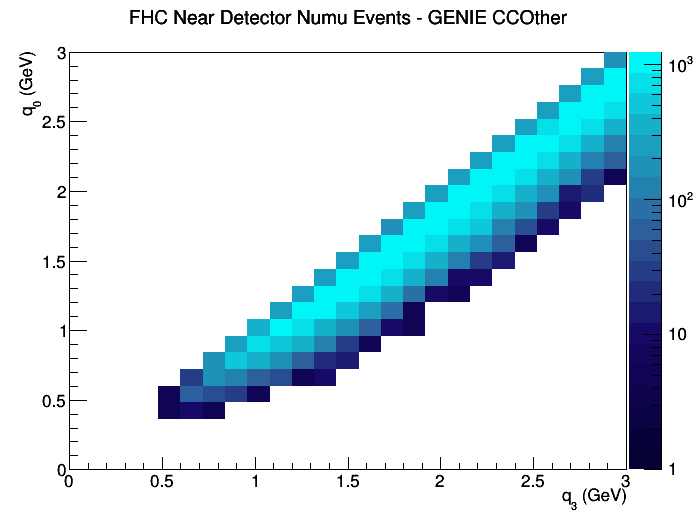
\includegraphics[width=\linewidth]{q0_q3/nominal/CCOther_FHC_ND_numu_q3_q0_GENIE.png}
%\endminipage
%\minipage{.3\textwidth}
%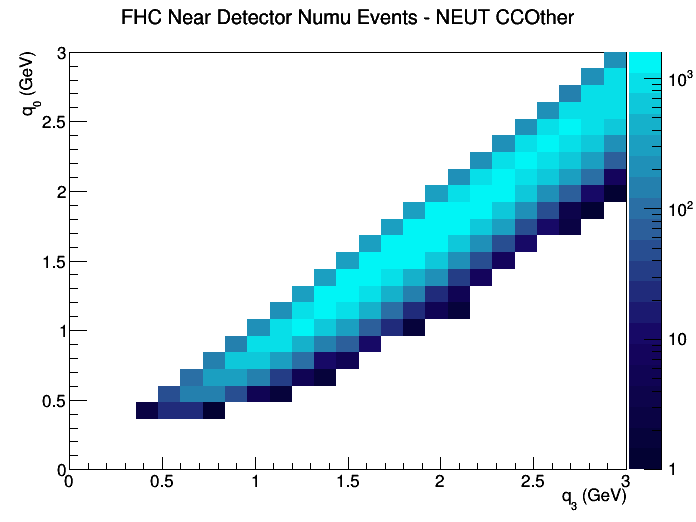
\includegraphics[width=\linewidth]{q0_q3/nominal/CCOther_FHC_ND_numu_q3_q0_NEUT.png}
%\endminipage
%\minipage{.3\textwidth}
%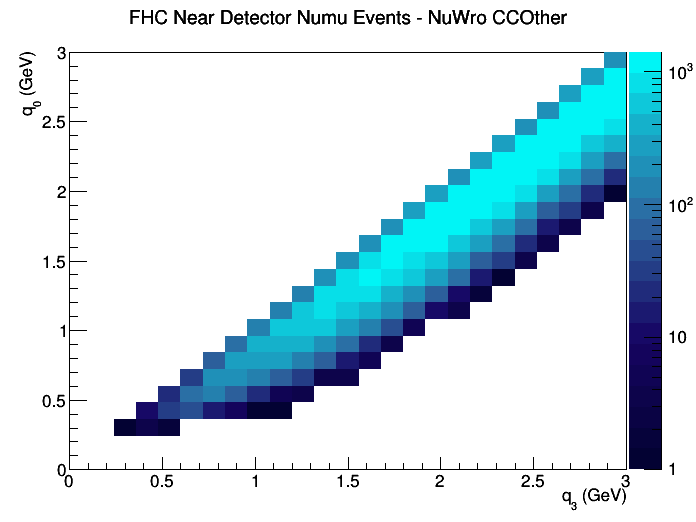
\includegraphics[width=\linewidth]{q0_q3/nominal/CCOther_FHC_ND_numu_q3_q0_NuWro.png}
%\endminipage
%\newline
%\minipage{.3\textwidth}
%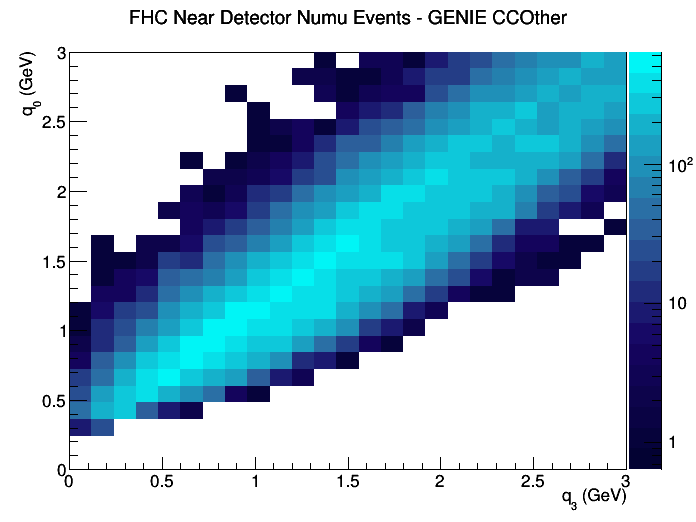
\includegraphics[width=\linewidth]{eff_q0_q3/FGT/CCOther_FHC_ND_numu_q3_q0_GENIE.png}
%\endminipage
%\minipage{.3\textwidth}
%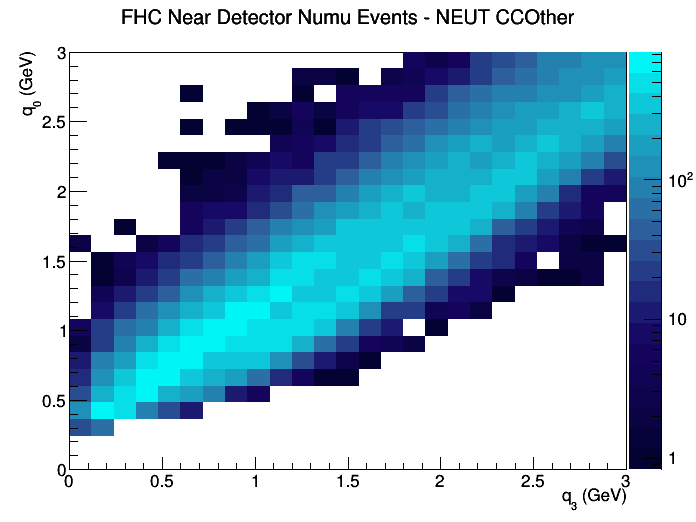
\includegraphics[width=\linewidth]{eff_q0_q3/FGT/CCOther_FHC_ND_numu_q3_q0_NEUT.png}
%\endminipage
%\minipage{.3\textwidth}
%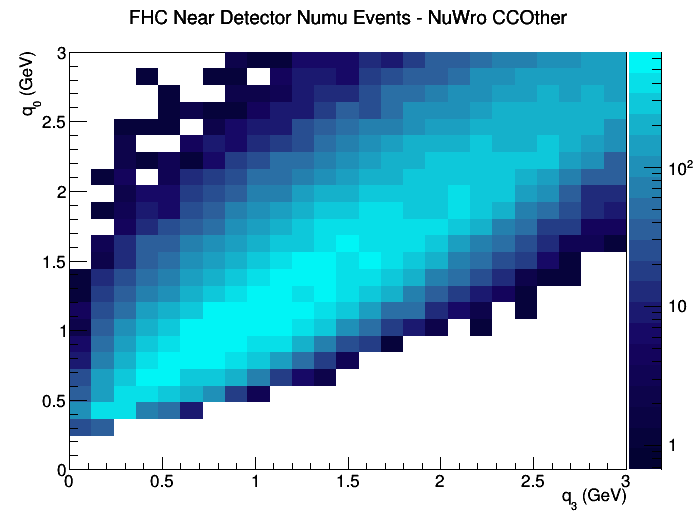
\includegraphics[width=\linewidth]{eff_q0_q3/FGT/CCOther_FHC_ND_numu_q3_q0_NuWro.png}
%\endminipage
%\caption{$q_0 \textrm{ - } q_3$ $\nu_{\mu}$ events using DUNE flux, Top Row: No Efficiencies applied, Bottom Row: FGT efficiencies applied to ND and LAr effiencies applied to FD. Right to Left: GENIE events distribution, NEUT events distribution, NuWro events distribution. The left $q_0 \textrm{ - } q_3$ region is being filled in after efficiencies are applied.}
%\label{fig:q0q3_numu_CCOther_events}
%\end{figure}
%\begin{figure}[h]
%\centering
%\minipage{.3\textwidth}
%\includegraphics[width=\linewidth]{Q2/nominal/CCOther_FHC_ND_numu_Q2_GENIE.png}
%\endminipage
%\minipage{.3\textwidth}
%\includegraphics[width=\linewidth]{Q2/nominal/CCOther_FHC_ND_numu_Q2_NEUT.png}
%\endminipage
%\minipage{.3\textwidth}
%\includegraphics[width=\linewidth]{Q2/nominal/CCOther_FHC_ND_numu_Q2_NuWro.png}
%\endminipage
%\newline
%\minipage{.3\textwidth}
%\includegraphics[width=\linewidth]{eff_Q2/FGT/CCOther_FHC_ND_numu_Q2_GENIE.png}
%\endminipage
%\minipage{.3\textwidth}
%\includegraphics[width=\linewidth]{eff_Q2/FGT/CCOther_FHC_ND_numu_Q2_NEUT.png}
%\endminipage
%\minipage{.3\textwidth}
%\includegraphics[width=\linewidth]{eff_Q2/FGT/CCOther_FHC_ND_numu_Q2_NuWro.png}
%\endminipage
%\caption{$Q^2$ events using DUNE flux, Top Row: No Efficiencies applied, Bottom Row: FGT efficiencies applied to ND and LAr effiencies applied to FD. Right to Left: GENIE events distribution, NEUT events distribution, NuWro events distribution. The low $Q^2$ region is being filled in after efficiencies are applied.}
%\label{fig:Q2_numu_CCOther_events}
%\end{figure}
%\FloatBarrier


\section{Reconstructed Energy}\label{sec:Reco}
%\subsection{Final State, Reconstructed Energy}

A framework for investigating variations in reconstructed energy calculations between different generators and ND configurations has been developed. %However, because it is calculated only by summing the final state energy (generator truth information), this is largely incomplete, and it serves only as a starting point for more robust studies. The full studies will include detector efficiencies and kinematic cuts to fully display the differences between models and configurations. 
Currently, the estimate for the incident neutrino energy is calculated by summing the total energy from final state leptons and pions (all charges) and the kinetic energy of final state protons after passing efficiencies through the data sets. All neutrons are assumed undetectable. 
This can be summed up in Equation~\ref{eq:ereco}:
%\begin{equation}
%E_{reco} = \Sigma {E_{lep}} + \Sigma E_{\pi} + \Sigma (E_{prot} - M_{prot})
%\label{eq:ereco}
%\end{equation}
where $E_{lep}$ is the energy of the outgoing lepton, $E_{\pi}$ is the energy of the pion, and $E_{prot}$ and $M_{prot}$ are the energy and mass of the proton.
%This is achieved by using the NUISANCE software package to reduce the output from various Monte Carlo neutrino event generators (including GENIE, NEUT, NUWRO, as well as the nuclear reaction and transport simulation software, GiBuu) into a common format that can easily be analyzed. 
%Work has begun to include tracking/PID efficiencies to accept or reject final state particles. So far, only the full information (barring $\pi^0$ efficiencies) for the FGT is available, but the inclusion of the LAr or GAr TPCs will be easily implemented. 

%\subsection{$E_\nu - E_{reco}$} 



\subsection{Neutron Multiplicities \& Energy}
\label{subsec:N_multiplicities_Energy}

Differences between models in the number of final state neutrons and the total energy into FS neutrons can largely affect reconstruction of neutrino energy. Large variations in reconstructed energy can arise due to missing energy caused by the inability to detect neutrons in the various models.  

To investigate this, we have looked at GENIE, NEUT, and NUWRO to see if the different models showed a large difference in the neutron energy and multiplicity.  
This was done for CCQE-like, CC1$\pi$, 2P2H, and everything else (``Other'') interactions and neutrinos as well as anti-neutrinos.  
In all cases, the generators agreed rather well with each other even though there were some differences in the neutron multiplicity. 
These differences only account for a small fraction of the events.
Figure~\ref{fig:Neutron_multi_2p2h_ND} shows an example of this for 2P2H neutrino events, while the other interaction modes can be found in Appendix~\ref{app:Neutron_Multiplicities}
  
\begin{figure}
\centering
\begin{subfigure}[b]{0.32\textwidth}
  \includegraphics[width=\textwidth]{nneutrons_v_total_ene/Nneutrons_Total_ENe_2p2h_GENIE_ND_numu.pdf}
\end{subfigure}
\begin{subfigure}[b]{0.32\textwidth}
  \includegraphics[width=\textwidth]{nneutrons_v_total_ene/Nneutrons_Total_ENe_2p2h_NEUT_ND_numu.pdf}
\end{subfigure}
\begin{subfigure}[b]{0.32\textwidth}
  \includegraphics[width=\textwidth]{nneutrons_v_total_ene/Nneutrons_Total_ENe_2p2h_NUWRO_ND_numu.pdf}
\end{subfigure}
\caption{The neutron multiplicity vs total neutron energy for 2P2H interactions for GENIE, NEUT, and NUWRO, respectively.  Even though they do show a different phase-space for the neutron multiplicity, they all agree where most of the energy lost to neutrons should be.  This is similar for other interaction types as well.}
\label{fig:Neutron_multi_2p2h_ND}
\end{figure}
Further more, the difference in the multiplicities between the generators becomes irrelevant after a ND to FD extraction, as can be seen in Figure~\ref{fig:Neutron_multi_2p2h_ND_FD}.
Here, the region where the most energy is lost agrees very well between the ND and FD for all generators and interaction types.
The areas with low statistics do show a disagreement, but very few events fall into this area.

\begin{figure}
\centering
\begin{subfigure}[b]{0.32\textwidth}
  \includegraphics[width=\textwidth]{nneutrons_v_total_ene/Nneutrons_Total_ENe_2p2h_GENIE_ND_FD_numu_norm.pdf}
\end{subfigure}
\begin{subfigure}[b]{0.32\textwidth}
  \includegraphics[width=\textwidth]{nneutrons_v_total_ene/Nneutrons_Total_ENe_2p2h_NEUT_ND_FD_numu_norm.pdf}
\end{subfigure}
\begin{subfigure}[b]{0.32\textwidth}
  \includegraphics[width=\textwidth]{nneutrons_v_total_ene/Nneutrons_Total_ENe_2p2h_NUWRO_ND_FD_numu_norm.pdf}
\end{subfigure}
\caption{The ratio of the ND to the FD for neutron multiplicity vs total neutron energy for 2P2H interactions for GENIE, NEUT, and NUWRO, respectively.  In the area where the largest amount of energy is lost to neutrons, low multiplicity and low energy, the agreement between the ND and FD is almost perfect.} 
\label{fig:Neutron_multi_2p2h_ND_FD}
\end{figure}
Care should still be taken when calculating the total neutrino of the event if only a calorimetric approach is used, as is the case in this document.
This is because as much as 50\% of the energy can be taken away by the neutron in CCQE-like events.
Even for 2P2H events, as shown in Figure~\ref{fig:Neutron_multi_ene_enu_2p2h_ND}, it can be as much as 30\%.
The other interaction modes and anti-neutrino events can also be found in Appendix~\ref{app:Neutron_Multiplicities} and have a smaller fraction.

\begin{figure}
\centering
\begin{subfigure}[b]{0.32\textwidth}
  \includegraphics[width=\textwidth]{nneutrons_ene_enu/Nneutrons_Enu_true_2p2h_GENIE_ND_numu_norm.pdf}
\end{subfigure}
\begin{subfigure}[b]{0.32\textwidth}
  \includegraphics[width=\textwidth]{nneutrons_ene_enu/Nneutrons_Enu_true_2p2h_NEUT_ND_numu_norm.pdf}
\end{subfigure}
\begin{subfigure}[b]{0.32\textwidth}
  \includegraphics[width=\textwidth]{nneutrons_ene_enu/Nneutrons_Enu_true_2p2h_NUWRO_ND_numu_norm.pdf}
\end{subfigure}
\caption{Neutron multiplicity vs total neutron energy divide by the neutrino energy for 2P2H interactions from GENIE, NEUT, and NUWRO, respectively.  For low multiplicity, the neutron carries away a significant fraction of the neutrino energy.} 
\label{fig:Neutron_multi_ene_enu_2p2h_ND}
\end{figure}
\FloatBarrier

 Additionally, investigations in the ability for errors in GENIE to cover the differences between models have been started. 

\subsection{Proton/Pion Multiplicity and Momentum}
\label{subsec:Particle_multiplicities_momentum}

Similar to the neutron multiplicity and energy studies, proton and pion mutliplicities and energies offer insight into the coupling of the detector configurations with variations in FSI models as well as the energy reconstruction capabilities of the different detector configurations. The total momentum of the particles gives us a proxy for the energy into the FS protons or pions as well as a direct link to detector efficiency effects.  For these studies, the 3-momentum of the final state (after efficiencies) protons or charged pions are summed. The magnitude is then plotted against the multiplicity for the specific particle type. This was done for the FS particles in true-CCQE, true-2p2h, CC0$\pi$, CC1$\pi$, and CCOther, and with all 3 ND configuration efficiencies and the LAr FD efficiencies, as well as with no efficiencies applied. As the efficiencies for pions are currently unknown for the LAr and GAr, we will only consider the protons in the current iteration of this note. Note that the LAr and GAr are still only naive assumptions.

 
\begin{figure}[h]
\minipage{.3\textwidth}
\includegraphics[width=\linewidth]{eff_N_P/FGT/protons/ratios/CCQE_NEUT_GENIE_numu_near_N_P.png}
\endminipage
\minipage{.3\textwidth}
\includegraphics[width=\linewidth]{eff_N_P/FGT/protons/ratios/CCQE_NEUT_GENIE_numu_far_N_P.png}
\endminipage
\minipage{.3\textwidth}
\includegraphics[width=\linewidth]{eff_N_P/FGT/protons/ratios/CCQE_NEUT_GENIE_numu_NF_N_P.png}
\endminipage
\caption{Nprotons vs. P protons distributed events using DUNE flux. Left: Ratio of NEUT to GENIE output at ND with FGT efficiencies, Mid: Ratio of NEUT to GENIE output at FD with LAr efficiencies, Right: Double ratio of NEUT to GENIE, Near to Far}
\end{figure}
\FloatBarrier
%\begin{equation}
%|\vec{P_{total,i}}| = |\Sigma \vec{P_i}|
%\end{equation}

\subsection{Difference from True Neutrino Energy}
\label{subsec:EDiff}
The studies in Sections~\ref{subsec:N_multiplicities_Energy} and ~\ref{subsec:Particle_multiplicities_momentum} highlight the differences in the generators in reproducing the true neutrino energy, as well as the differences in the abilities of the different detector configurations to reconstruct this energy. This section studies the overall change we see to $E_{reco}$ as we apply detector efficiencies. To do this, the difference between true and reconstructed neutrino energy from each generator is plotted. Each distribution is normalized to 1 so the y-axis serves as the relative event rate. This is done separately for a 'perfect' near detector - one in which we assume no particles except neutrons are rejected - and each near detector configuration and the far detector with simple LAr thresholds for protons, as well for each interaction type: true-CCQE, true-2p2h, CC0$\pi$, CC1$\pi$, and CCOther. True-CCQE and true-2p2h are both defined as MC-level CCQE/2p2h interaction with 1 reconstructed lepton if efficiencies are applied. CC0$\pi$ is defined as 0 $\pi^{\pm}$, 1 lepton, and any number of protons and $\pi^0$ after reconstruction. CC1$\pi$ is defined as 1 $\pi^{\pm}$, 1 lepton, and any number of protons and $\pi^0$ after reconstruction. Finally, CCOther is defined as any final state with 1 lepton and any number of hadrons reconstructed.

In $\nu_\mu$ mode: for all reaction types except CCOther, all three generators seem to have similar differences in all detector configurations. This is evident in Figure~\ref{fig:numu_Etrue_ereco_FGT_CCQE_and_CCOther} - which includes CCQE and CCOther interactions in the ND with FGT efficiencies - and the figures in Appendix~\ref{app:Ereco_app}. For CCOther, all three generators appear to have a long tail extending to high discrepancy regions - well past that of CCQE for example - though NuWro has a higher amount of events in the $\Delta E$ = 0.5 GeV to 2 GeV region. 
\begin{figure}[h]
\centering
\minipage{.32\textwidth}
\includegraphics[width=\linewidth]{Ereco_Etrue/numu_FGT_CCQE.png}
\endminipage
\minipage{.32\textwidth}
\includegraphics[width=\linewidth]{Ereco_Etrue/numu_FGT_CCOther.png}
\endminipage
\caption{Difference between true and reconstructed Neutrino Energy in the FGT ND. CCQE events seem to have similar discrepancies, while CCOther mode has large tails in all three generators with NuWro having more events with higher discrepancy than the other two. }
\label{fig:numu_Etrue_ereco_FGT_CCQE_and_CCOther}
\end{figure}
\FloatBarrier

Meanwhile, for $\overline{\nu_\mu}$ CCQE, 2p2h, and CC0$\pi$ events NuWro consistently has $\Delta E$ closer to 0 than the other generators as shown in Figure~\ref{fig:numubar_Etrue_ereco_FGT_CCQE_2p2h_CC0Pi}. In CC1$\pi$ and CCOther NuWro again has more events where true neutrino energy is underestimated by reconstruction, shown in Figure~\ref{fig:numubar_Etrue_ereco_FGT_CC1Pi_CCOther}. Additionally, there exists a large difference in the distribution of events from NEUT and NuWro between the FGT and LAr FD. This is slightly better in the LAr ND - as expected due to our naive LAr efficiencies. This can be seen in Figure~\ref{fig:numubar_Etrue_ereco_CCOther_diffs}.
\begin{figure}[h]
\centering
\minipage{.3\textwidth}
\includegraphics[width=\linewidth]{Ereco_Etrue/numubar_FGT_CCQE.png}
\endminipage
\minipage{.3\textwidth}
\includegraphics[width=\linewidth]{Ereco_Etrue/numubar_FGT_2p2h.png}
\endminipage
\minipage{.3\textwidth}
\includegraphics[width=\linewidth]{Ereco_Etrue/numubar_FGT_CC0Pi.png}
\endminipage
\newline
\minipage{.3\textwidth}
\includegraphics[width=\linewidth]{Ereco_Etrue/numubar_FD_CCQE.png}
\endminipage
\minipage{.3\textwidth}
\includegraphics[width=\linewidth]{Ereco_Etrue/numubar_FD_2p2h.png}
\endminipage
\minipage{.3\textwidth}
\includegraphics[width=\linewidth]{Ereco_Etrue/numubar_FD_CC0Pi.png}
\endminipage
\caption{Difference between true and reconstructed $E_\nu$. Top: At Near Detector with FGT efficiencies. Bottom: Far Detector with LAr efficiencies. Left to Right: CCQE, 2p2h, CC0$\pi$. NuWro can be seen to have consistently less discrepancy in reconstructed energy than NEUT and GENIE in CCQE, 2p2h, and CC0$\pi$. }
\label{fig:numubar_Etrue_ereco_FGT_CCQE_2p2h_CC0Pi}
\end{figure}
\begin{figure}[h]
\centering
\minipage{.5\textwidth}
\includegraphics[width=\linewidth]{Ereco_Etrue/numubar_FGT_CC1Pi.png}
\endminipage
\minipage{.5\textwidth}
\includegraphics[width=\linewidth]{Ereco_Etrue/numubar_FGT_CCOther.png}
\endminipage
\caption{NuWro has higher discrepancy in reconstructed energy than NEUT and GENIE in both CC1$\pi$ and CCOther.}
\label{fig:numubar_Etrue_ereco_FGT_CC1Pi_CCOther}
\end{figure}
\begin{figure}[h]
\centering
\minipage{.3\textwidth}
\includegraphics[width=\linewidth]{Ereco_Etrue/numubar_FD_CCOther.png}
\endminipage
\minipage{.3\textwidth}
\includegraphics[width=\linewidth]{Ereco_Etrue/numubar_FGT_CCOther.png}
\endminipage
\minipage{.3\textwidth}
\includegraphics[width=\linewidth]{Ereco_Etrue/numubar_LAr_CCOther.png}
\endminipage
\caption{NuWro CCOther events have differences in shape between the Far Detector and LAr FD. The LAr ND matches more closely, though this is expected because of our current naive efficiency assumptions.}
\label{fig:numubar_Etrue_ereco_CCOther_diffs}
\end{figure}
\FloatBarrier

%As a first check in the ability to reconstruct neutrino energy, I began investigating the differences between the total final state energy and initial state energy. I've verified with Callum that the NUISANCE framework successfully treats the particle stacks from the various generators, and any differences come from how the different generators handle FSI. 


% \subsection{Nucleon multiplicity vs. W}
% \label{sec:Nucleon_multi_w}
% Differences in mapping from $E_{reco}$ to true variables can arise from shape differences in nucleon multiplicities vs. W distributions. 
% These distributions can also show where in the phase space most of the events shown in Section~\ref{sec:N_multiplicities_Energy} and Section~\ref{sec:Particle_multiplicities_Energy} exist.  A first look of this is shown in this section.

% \subsubsection{Neutrons vs W}

% Apart from the difference in neutron multiplicity discussed in Section~\ref{sec:N_multiplicities_Energy}, the exact phase space of these event in the neutron/W plane is slightly different.  
% This is most pronounced for 2P2H events, as can be seen in Figure~\ref{Neutron_w_2p2h_ND}. 
% The width of NEUT's peak is broader then GENIE's or NUWRO's while NUWRO allows for much higher W's.

% \begin{figure}
% \centering
% \begin{subfigure}[b]{0.32\textwidth}
%   \includegraphics[width=\textwidth]{nneutrons_w/Nneutrons_W_nuc_rest_2p2h_GENIE_ND_numu.pdf}
% \end{subfigure}
% \begin{subfigure}[b]{0.32\textwidth}
%   \includegraphics[width=\textwidth]{nneutrons_w/Nneutrons_W_nuc_rest_2p2h_NEUT_ND_numu.pdf}
% \end{subfigure}
% \begin{subfigure}[b]{0.32\textwidth}
%   \includegraphics[width=\textwidth]{nneutrons_w/Nneutrons_W_nuc_rest_2p2h_NUWRO_ND_numu.pdf}
% \end{subfigure}
% \caption{The neutron multiplicity vs W for 2P2H interactions from GENIE, NEUT, and NUWRO, respectively.  It can be seen that all three event generators have the peak of the distribution at the same place, but NEUT's peak is much broader while NUWRO allows for much higher W's.}
% \label{fig:Neutron_w_2p2h_ND}
% \end{figure}

% However, Figure~\ref{fig:Neutron_w_2p2h_ND_FD} shows that the differences are not so important if a near to far extrapolation is used, as both the ND and FD have simular responses.
% To see if the different models could have a larger affect on the physics results, we have taken a double ratio of the ND/FD and the different generators to GENIE.  
% Interestingly, Figure~\ref{fig:Neutron_w_2p2h_ND_FD_GENIE} indicates that there would not be large affect if a few perecent difference between the models is acceptable.

% \begin{figure}
% \centering
% \begin{subfigure}[b]{0.32\textwidth}
%   \includegraphics[width=\textwidth]{nneutrons_w/Nneutrons_W_nuc_rest_2p2h_GENIE_ND_FD_numu_norm.pdf}
% \end{subfigure}
% \begin{subfigure}[b]{0.32\textwidth}
%   \includegraphics[width=\textwidth]{nneutrons_w/Nneutrons_W_nuc_rest_2p2h_NEUT_ND_FD_numu_norm.pdf}
% \end{subfigure}
% \begin{subfigure}[b]{0.32\textwidth}
%   \includegraphics[width=\textwidth]{nneutrons_w/Nneutrons_W_nuc_rest_2p2h_NUWRO_ND_FD_numu_norm.pdf}
% \end{subfigure}
% \caption{The ND/FD ratio of neutron multiplicity vs W for 2P2H interactions from GENIE, NEUT, and NUWRO, respectively.  The effects of the different phase space seen in Figure~\ref{fig:Neutron_w_2p2h_ND} is not great if a ND ro FD extropolation is used.  This can be seen by the ratio being very close to one at the peak of Figure~\ref{fig:Neutron_w_2p2h_ND} distribution.}
% \label{fig:Neutron_w_2p2h_ND_FD}
% \end{figure}

% These results are also true for protons and pions, though pions have a much lower multiplicity.  
% Those results, along with other interactions can be found in Appendix~\ref{app:Nucleon_W}.

% \begin{figure}
% \centering
% \begin{subfigure}[b]{0.32\textwidth}
%   \includegraphics[width=\textwidth]{nneutrons_w/Nneutrons_W_nuc_rest_2p2h_GENIE_NEUT_ND_FD_numu_norm.pdf}
% \end{subfigure}
% \begin{subfigure}[b]{0.32\textwidth}
%   \includegraphics[width=\textwidth]{nneutrons_w/Nneutrons_W_nuc_rest_2p2h_GENIE_NUWRO_ND_FD_numu_norm.pdf}
% \end{subfigure}
% \caption{The double ratio of ND/FD and the event generators to GENIE of the neutron multiplicity vs W for 2P2H interactions.  Despite the differences seen in the W distributions, the double ratio shows suprisingly good agreement between the generators, indicating that the different models should not have a large impact on the final results.}
% \label{fig:Neutron_w_2p2h_ND_FD_GENIE}
% \end{figure}

% \subsubsection{Protons vs W}

% In the last section we saw a differnce in the phase space between the different generators.  
% Now we will show an instance where the phase space is almost the same but there is a large difference between the ND and FD.  
% Though here we are only showing the results for CC1$\pi$ via protons, the results are the same for CC-Other (anything not CCQE, CC1$\pi$, or 2P2H), and neutrons along with pions.
% Figure~\ref{fig:Proton_w_res_ND} shows that GENIE, NEUT, and NUWRO have very similar distributions.

% \begin{figure}
% \centering
% \begin{subfigure}[b]{0.32\textwidth}
%   \includegraphics[width=\textwidth]{nprotons_w/Nprotons_W_nuc_rest_res_GENIE_ND_numu.pdf}
% \end{subfigure}
% \begin{subfigure}[b]{0.32\textwidth}
%   \includegraphics[width=\textwidth]{nprotons_w/Nprotons_W_nuc_rest_res_NEUT_ND_numu.pdf}
% \end{subfigure}
% \begin{subfigure}[b]{0.32\textwidth}
%   \includegraphics[width=\textwidth]{nprotons_w/Nprotons_W_nuc_rest_res_NUWRO_ND_numu.pdf}
% \end{subfigure}
% \caption{The proton multiplicity vs W for CC1$\pi$ interactions from GENIE, NEUT, and NUWRO, respectively.  It can be seen that all three event generators have the peak of their distribution at the same place and are almost identical}
% \label{fig:Proton_w_res_ND}
% \end{figure}

% If a near to far detector extrapolation is used, however, there are much larger differences in region of most interest. 
% Figure~\ref{fig:Proton_w_res_ND_FD} shows that there is a difference between the two detectors between 20\% and 40\% at the peak of the distribution.  
% There is also a clear difference in lower W values compared to higher W values. 


% \begin{figure}
% \centering
% \begin{subfigure}[b]{0.32\textwidth}
%   \includegraphics[width=\textwidth]{nprotons_w/Nprotons_W_nuc_rest_res_GENIE_ND_FD_numu_norm.pdf}
% \end{subfigure}
% \begin{subfigure}[b]{0.32\textwidth}
%   \includegraphics[width=\textwidth]{nprotons_w/Nprotons_W_nuc_rest_res_NEUT_ND_FD_numu_norm.pdf}
% \end{subfigure}
% \begin{subfigure}[b]{0.32\textwidth}
%   \includegraphics[width=\textwidth]{nprotons_w/Nprotons_W_nuc_rest_res_NUWRO_ND_FD_numu_norm.pdf}
% \end{subfigure}
% \caption{The ND/FD ratio of the proton multiplicity vs W for CC1$\pi$ interactions from GENIE, NEUT, and NUWRO, respectively.  Unlike with 2P2H events shown for neutrons, there are clear differences between the ND and FD.  At the peak of the distribution this is between 20\% and 40\%.  Furthermore, there is a clear difference between W values below 2000 and ones above it.}
% \label{fig:Proton_w_res_ND_FD}
% \end{figure}

% We can again see if the different models could have a larger affect on the physics results, by taking the double ratio as we did before.
% Simular to before, Figure~\ref{fig:Proton_w_res_ND_FD_GENIE} indicates that there would not be large affect if a few perecent difference between the models is acceptable.
% In the region of interest, the difference between GENIE and NEUT is negligable while it is small compared to NUWRO.


% \begin{figure}
% \centering
% \begin{subfigure}[b]{0.32\textwidth}
%   \includegraphics[width=\textwidth]{nprotons_w/Nprotons_W_nuc_rest_res_GENIE_NEUT_ND_FD_numu_norm.pdf}
% \end{subfigure}
% \begin{subfigure}[b]{0.32\textwidth}
%   \includegraphics[width=\textwidth]{nprotons_w/Nprotons_W_nuc_rest_res_GENIE_NUWRO_ND_FD_numu_norm.pdf}
% \end{subfigure}
% \caption{The double ratio of ND/FD and the event generators to GENIE of the proton multiplicity vs W for CC1$\pi$ interactions.  Despite the differences seen in the single ratio, the double ratio shows suprisingly good agreement between the generators}
% \label{fig:Proton_w_res_ND_FD_GENIE}
% \end{figure}



\section{Future Work}\label{sec:Future}

The above studies need to be furthered and expanded upon to successfully arrive at useful conclusions on ND configuration choice. 

\begin{itemize}

\item Improved statistics.
	\begin{itemize}
		\item This can be easily and quickly achieved.
	\end{itemize}
\item Investigate origins of high-$Q^2$ variations
	\begin{itemize}
		\item Is this FSI or detector effects?
	\end{itemize}
\item Extend studies to include LAr and GAr efficiency and acceptance information when available.
\item Extend final state studies into proton multiplicity vs. energy, and include pions when efficiencies are available.
%\item Current uncertainties are invariant of target choice. Need to extend studies to include Calcium-40 target for FGT studies
%\item Include a mapping of $E_{true}$ to $E_{reco}$ along with $y_{true}$ to $y_{reco}$ and investigate differences between configurations.

\end{itemize}


%\subsection{Ereco, yreco}
%An additional study to be commenced is the mapping from Ereco \& yreco into other kinematic variables (i.e. $Q^2$, $q_0$ vs. $q_3$), and the ability to similarly map model variations.
\appendix

%\subfile{Appendix_Neutron_Multi.tex}
%
%\subfile{Appendix_Nucleon_Multi.tex}
%
%\subfile{DUNE_appendix_Ereco_plots.tex}
%\subfile{DUNE_appendix_Q2_plots.tex}
%\subfile{DUNE_appendix_q0_q3_plots.tex}
%\subfile{DUNE_appendix_N_P_plots_protons.tex}

\begin{thebibliography}{7}

\bibitem{DUNE_CDR1}
The DUNE Collaboration
\textit{Long-Baseline Neutrino Facility (LBNF) and Deep Underground Neutrino Experiment (DUNE) Conceptual Design Report Volume 1: The LBNF and DUNE Projects}
arXiv:1601.05471v1

\bibitem{DUNE_review}
Maury Goodman
\textit{The Deep Underground Neutrino Experiment}
Advances in High Energy Physics, vol. 2015, Article ID 256351, 9 pages, 2015. doi:10.1155/2015/256351

\bibitem{GENIE}
Andreopoulos, C. \textit{et al}.
\textit{The GENIE Neutrino Monte Carlo Generator}.
Nucl.Instrum.Meth. A614 (2010) 87-104 arXiv:0905.2517 [hep-ph] FERMILAB-PUB-09-418-CD

\bibitem{NEUT}
Hayato, Yoshinari 
\textit{A neutrino interaction simulation program library NEUT}.
Acta Phys.Polon. B40 (2009) 2477-2489

\bibitem{NUWRO}
T. Golan, J.T. Sobczyk, J. Zmuda
\textit{NuWro: the Wrocław Monte Carlo Generator of Neutrino Interactions}.
Nuclear Physics B - Proceedings Supplements 229 (2012) 499

\bibitem{NUISANCE}
P. Stowell, C. Wret, C. Wilkinson, L. Pickering, S. Cartwright, Y. Hayato, K. Mahn, K.S. McFarland, J. Sobczyk, R. Terri, L. Thompson, M.O. Wascko, Y. Uchida
\textit{NUISANCE: a neutrino cross-section generator tuning and comparison framework}
arXiv:1612:07393v2

\bibitem{VALOR}
Andreopoulos, \textit{et al.}
\textit{VALOR DUNE Joint Oscillation and Systematics Constraint Fit}


\end{thebibliography}

\end{document}




